\documentclass[12pt]{memoir}

\def\nsemestre {I}
\def\nterm {Spring}
\def\nyear {2023}
\def\nprofesor {Maria Gillespie}
\def\nsigla {MATH502}
\def\nsiglahead {Combinatorics 2}
\def\nextra {P}
\def\nlang {ENG}

\makeatletter
\ifx \nauthor\undefined
  \def\nauthor{Ignacio Rojas}
\else
\fi

\ifx \nextra \undefined
\ifx \nlang \undefined
\author{Basado en las clases impartidas por \nprofesor \\\small Notas tomadas por \nauthor}
\else
\author{Based on the lectures by \nprofesor \\\small Notes written by \nauthor}
\fi
\else
\author{\nauthor}
\fi
\date{\nterm\ \nyear}

%%%%%%%%%%%%%
%% 1. Pacotes
%%%%%%%%%%%%%

\usepackage{alltt}
\usepackage{amsfonts}
\usepackage{amsmath}
\usepackage{amssymb}
\usepackage{amsthm}
\usepackage{algorithm}
\usepackage[noend]{algpseudocode}
\usepackage{array}
\newcommand\hmmax{0} % default 3
\newcommand\bmmax{0} % default 4 %%tex.se/3676,219310
%\usepackage{bbold}
\usepackage{bm}
\usepackage{booktabs}
%\usepackage{caption}
%\usepackage{cancel}
%\usepackage{dsfont}
\usepackage{esint}
\usepackage{fancyhdr}
\usepackage{graphicx}
\usepackage[utf8]{inputenc}
\usepackage{listings}
\usepackage{mathabx}
\usepackage[cal=euler]{mathalfa}
%\usepackage[cal=euler,frak=euler]{mathalfa} % mathcal (JIRR) precisabamos correr initexmf --mkmaps en cmd JCVDG
\usepackage{mathdots}
\usepackage{mathrsfs}
%\usepackage{mathtools}
\usepackage{microtype}
\usepackage{multicol}
\usepackage{multirow}
\usepackage[theoremfont,largesc,tighter,osf]{newpxtext} %JCV Diff
\let\widering\undefined
%\usepackage[bigdelims,vvarbb]{newpxmath} %JCVDG
%por alguna razón esto afectaba las tildes en \min, \lim y demás
%\usepackage{pdflscape}
\usepackage{pgfplots}
\usepackage{physics}
\usepackage{siunitx}
\usepackage{slashed}
%\usepackage{stmaryrd}
%\SetSymbolFont{stmry}{bold}{U}{stmry}{m}{n}
%\usepackage{subfigure}
\usepackage{subcaption}
\usepackage{tabularx}
\usepackage[breakable,skins]{tcolorbox}
\usepackage{textcomp} %%JCVDG
\usepackage{tikz}
\usepackage{tkz-euclide}
\usepackage[normalem]{ulem}
\usepackage[all]{xy}
\usepackage{imakeidx}
\ifx \nlang \undefined
\usepackage[spanish]{babel}
\else\fi 
\usepackage{wrapfig}

%%%%%%%%%%%%%%%%%%%%
%% 2. Document Setup
%%%%%%%%%%%%%%%%%%%%

\ifx \nextra \undefined
    \ifx \nlang \undefined
    \makeindex[intoc, title=Índice Analítico] %Título de índice analítico
    %El índice general es aquel en el que se indican los capítulos, títulos y subtítulos del libro.
    %Índice onomástico es donde aparece el nombre de personas mencionadas en el texto, por orden alfabético con el número de las páginas donde aparecen.
    %El índice analítico se refiere a los temas y conceptos que aparecen en el libro
    \indexsetup{othercode={\fancyhead[LE]{\emph{Índice Analítico}}}}
    \else
    \makeindex[intoc, title=Index] 
    \indexsetup{othercode={\fancyhead[LE]{\emph{Index}}}}
    \fi
  \usepackage[pdftex,
    hidelinks,
    pdfauthor={\nauthor},
    pdfsubject={Notas: \nsiglahead\ \nsemestre-\nyear},
    pdftitle={Semestre \nsemestre\ - \nsigla},
  pdfkeywords={UCR Costa Rica Matem\'aticas Mate \nsemestre\ \nterm\ \nyear\ \nsiglahead}]{hyperref}
  \title{\nsigla\ --- \nsiglahead}
\else
  \usepackage[pdftex,
     hidelinks,
    pdfauthor={\nauthor},
    pdfsubject={\nextra \nsiglahead\ \nsemestre-\nyear},
    pdftitle={Semestre \nsemestre\ - \nsigla},
  pdfkeywords={UCR Costa Rica Matem\'aticas Mate \nsemestre\ \nterm\ \nyear\ \nsiglahead\ \nextra}]{hyperref}

  \title{\nsigla\ --- \nsiglahead \\ {\Large \nextra}}
  \renewcommand\printindex{}
\fi

\pgfplotsset{compat=1.12}


\pagestyle{fancy}
\setlength{\headheight}{15.72pt} %preceding warning said make it at least this


\ifx \nsiglahead \undefined
\def\nsiglahead{\nsigla}
\fi

\lhead{} %%%empty lhead
\rfoot{\thepage}

\ifx \nextra \undefined
  \chead{
    \ifnum\thepage=1
    \else
      \ifx \nlang \undefined
      \textbf{Notas \nsiglahead\ \nsemestre-\nyear}
      \else
      \textbf{Notes \nsiglahead\ \nsemestre-\nyear}
      \fi
    \fi}
  \rhead{}%\firstxmark} % Top right header
\else
%    \chead{
%    \ifnum\thepage=1
%    \else
%      \textbf{Notas \nsiglahead\ \nsemestre-\nyear \ (\nextra)}
%    \fi}
     \chead{
       \textbf{\nextra\ \nsigla\ \nsemestre-\nyear}
     }
     \rhead{
       \textbf{\nauthor}
     }
\fi
\lfoot{}%\lastxmark} % Bottom left footer
\cfoot{} % Bottom center footer

\usetikzlibrary{arrows.meta}
\usetikzlibrary{decorations.markings}
\usetikzlibrary{decorations.pathmorphing}
\usetikzlibrary{positioning}
\usetikzlibrary{fadings}
\usetikzlibrary{intersections}
\usetikzlibrary{cd}

\ifx \nhtml \undefined
\else
  \renewcommand\printindex{}
  \DisableLigatures[f]{family = *}
  \let\Contentsline\contentsline
  \renewcommand\contentsline[3]{\Contentsline{#1}{#2}{}}
  \renewcommand{\@dotsep}{10000}
  \newlength\currentparindent
  \setlength\currentparindent\parindent

  \newcommand\@minipagerestore{\setlength{\parindent}{\currentparindent}}
  \usepackage[active,tightpage,pdftex]{preview}
  \renewcommand{\PreviewBorder}{0.1cm}

  \newenvironment{stretchpage}%
  {\begin{preview}\begin{minipage}{\hsize}}%
    {\end{minipage}\end{preview}}
  \AtBeginDocument{\begin{stretchpage}}
  \AtEndDocument{\end{stretchpage}}

  \newcommand{\@@newpage}{\end{stretchpage}\begin{stretchpage}}

  \let\@real@section\section
  \renewcommand{\section}{\@@newpage\@real@section}
  \let\@real@subsection\subsection
  \renewcommand{\subsection}{\@ifstar{\@real@subsection*}{\@@newpage\@real@subsection}}
\fi
\ifx \ntrim \undefined
\usepackage[shortlabels]{enumitem} %mfw package order matters por savetrees
\else
  \usepackage{geometry}
  \geometry{
    papersize={379pt, 699pt},
    textwidth=345pt,
    textheight=596pt,
    left=17pt,
    top=54pt,
    right=17pt
  }
  \headwidth=345pt
 \usepackage[extreme]{savetrees}
\fi

\ifx \darktheme\undefined
\else
\pagecolor[rgb]{0.2,0.231,0.302}%{0.23,0.258,0.321}
\color[rgb]{1,1,1}
\fi

\ifx \nextra \undefined
\let\@real@maketitle\maketitle
\renewcommand{\maketitle}{\@real@maketitle\begin{center}\begin{minipage}[c]{0.9\textwidth}\centering\footnotesize 
  \ifx \nlang \undefined
  Estas notas no están respaldadas por los profesores y han sido modificadas (a menudo de manera significativa) después de las clases. No están lejos de ser representaciones precisas de lo que realmente se dio en clase y en particular todos los errores son casi seguramente míos.
  \else 
  Please note that these notes were not provided or endorsed by the lecturer and have been significantly altered after the class. They may not accurately reflect the content covered in class and any errors are solely my responsibility.
  \fi
\end{minipage}\end{center}}
\else
\fi

\def\moverlay{\mathpalette\mov@rlay}
\def\mov@rlay#1#2{\leavevmode\vtop{%
   \baselineskip\z@skip \lineskiplimit-\maxdimen
   \ialign{\hfil$\m@th#1##$\hfil\cr#2\crcr}}}
\newcommand{\charfusion}[3][\mathord]{
    #1{\ifx#1\mathop\vphantom{#2}\fi
        \mathpalette\mov@rlay{#2\cr#3}
      }
    \ifx#1\mathop\expandafter\displaylimits\fi}

%%%%%%%%%%%%%%%%%%%%%%%%%%%%%%
%% 2.1 Some internal machinery
%%%%%%%%%%%%%%%%%%%%%%%%%%%%%%

\makeatletter
\renewcommand{\section}{\@startsection{section}{1}{\z@}%
							 {-3.25ex \@plus -1ex \@minus -.2ex}%
							 {1.5ex \@plus.2ex}%
							 {\normalfont\large\bfseries}}
\renewcommand{\subsection}{\@startsection{subsection}{2}{\z@}%
							 {-3.25ex \@plus -1ex \@minus -.2ex}%
							 {1.5ex \@plus .2ex}%
               {\normalfont\normalsize\bfseries}}
\newcommand*{\defeq}{\!\mathrel{\rlap{%
             \raisebox{0.3ex}{$\m@th\cdot$}}%
             \raisebox{-0.3ex}{$\m@th\cdot$}}%
                    =\!}
\makeatother
\ifx\ntrim\undefined
\newcommand{\coursetitle}{\nsigla: \nsiglahead}
\ifx\nextra\undefined
\pagestyle{ruled}
\makeoddhead{ruled}{\coursetitle}{}{\rightmark}
\else\fi
\settypeblocksize{49pc}{37pc}{*}
\setlrmargins{*}{*}{1.2}
\setulmargins{*}{*}{0.8}
\setheadfoot{16pt}{30pt}
\setheaderspaces{*}{1.5pc}{1}
\setmarginnotes{1pt}{1pt}{1pt}
\checkandfixthelayout

\setlength{\unitlength}{3pt}
\setlength{\hfuzz}{1pt}

\setlength{\fboxsep}{6pt}

\setlength{\footskip}{17pt}

\linespread{1.1}
\else\fi
\renewcommand{\cftdotsep}{\cftnodots} %%% no dots in ToC
\setpnumwidth{2em}  %%% width of page-number box in ToC


\newcommand{\stophere}{\relax} %% can be changed to `\endinput'
% \newcommand{\stophere}{\endinput} %% can be changed to `\relax'


\DeclareRobustCommand{\qned}{\ifmmode
  \else \leavevmode\unskip\penalty9999 \hbox{}\nobreak\hfill \fi
  \quad\hbox{\qnedsymbol}}
\newcommand{\qnedsymbol}{$\boxminus$} %% No-proofs end with `\qned'

\DeclareRobustCommand{\qef}{\ifmmode
  \else \leavevmode\unskip\penalty9999 \hbox{}\nobreak\hfill \fi
  \quad\hbox{\qefsymbol}}
\newcommand{\qefsymbol}{$\lozenge$} %% Examples end with `\qef'
\def\enddefn{\qef\endtrivlist}      %% `\qef' automático en defns
\def\endejem{\qef\endtrivlist}      %% `\qef' automático en ejemplos

\newcommand{\hideqed}{\renewcommand{\qed}{}} %% to suppress `\qed'
\newcommand{\hideqef}{\renewcommand{\qef}{}} %% to suppress `\qef'

% \newcommand{\ldbrack}{\ensuremath{[\mskip-2.5mu[}} %% corchetes [[
% \newcommand{\rdbrack}{\ensuremath{]\mskip-2.5mu]}} %% corchetes ]]

\newcommand{\stroke}{\mathbin|}     %% (for `\bbraket' and such)

\newcommand{\rtri}{\blacktriangleright} %% (for `\marker' and such)
\newcommand{\tribar}{|\mkern-2mu|\mkern-2mu|} %% norma triple: |||


%% Formatting changes:

\renewcommand{\labelitemi}{$\diamond$} %% instead of bullets

\renewcommand{\theenumi}{\alph{enumi}}  %% use lowercase letters
\renewcommand{\labelenumi}{\textup{(\theenumi)}} %% inside parentheses

%%%%%%%%%%%%%%
%% 2.2. Colors
%%%%%%%%%%%%%%

\definecolor{MATLABgreen}{RGB}{28,172,0} % color values Red, Green, Blue
\definecolor{MATLABlila}{RGB}{170,55,241}
\definecolor{dankBlue}{RGB}{51,60,77} % color values Red, Green, Blue
\definecolor{dankBlueLite}{RGB}{82,97,125} % color values Red, Green, Blue
\definecolor{celesUCR}{RGB}{0,192,243}
\definecolor{azulUCR}{RGB}{0,93,164}
\definecolor{verdeUCR}{RGB}{109,192,103}
\definecolor{yelloUCR}{RGB}{255,224,106}

%%%%%%%%%%%%%%%%%%%%%%%%%%%
%% 3. Theorems and suchlike
%%%%%%%%%%%%%%%%%%%%%%%%%%%

\ifx\nlang\undefined

\theoremstyle{plain}
\ifx \nextra \undefined
\newtheorem{Th}{Teorema}[section]      %%% Theorem 1.1.1
\newtheorem{Tmon}[Th]{Teoremón}
\newtheorem{Prop}[Th]{Proposición}     %%% Proposition 1.1.2
\newtheorem{Lem}[Th]{Lema}             %%% Lemma 1.1.3
\newtheorem{Cor}[Th]{Corolario}        %%% Corollary 1.1.4
\else
\newtheorem{Th}{Teorema}               %%% Theorem 1.1.1
\newtheorem{Tmon}{Teoremón}
\newtheorem{Prop}{Proposición}         %%% Proposition 1.1.2
\newtheorem{Lem}{Lema}                 %%% Lemma 3
\newtheorem{Cor}{Corolario}            %%% Corollary 4
\fi
\newtheorem*{nonum-Th}{Teorema}        %%% No-numbered Theorem
\newtheorem*{nonum-Cor}{Corolario}     %%% No-numbered Corollary

\theoremstyle{definition}
\ifx \nextra \undefined
\newtheorem{Def}[Th]{Definición}       %%% Definition 1.1.5
\newtheorem{Ex}[Th]{Ejemplo}           %%% Example 1.1.6
\newtheorem{Ej}[Th]{Ejercicio}         %%% Ejercicio 1.1.7
\else
\newtheorem{Def}{Definición}           %%% Definition 5
\newtheorem{Ex}{Ejemplo}               %%% Example 6
\newtheorem{Ej}{Ejercicio}             %%% Ejercicio 7
\fi
\newtheorem{Hec}[Th]{Hecho}            %%% Hecho 1.1.8
\newtheorem*{nonum-Def}{Definición}    %%% No number Definition
\newtheorem*{nonum-Ex}{Ejemplo}        %%% No number Example
\newtheorem*{nonum-Ej}{Ejercicio}      %%% No number Ejercicio
\newtheorem*{nonum-Hec}{Hecho}         %%% No number Fact


\theoremstyle{remark}
\newtheorem{Rmk}[Th]{Observación}      %%%Remark 1.1.9
\newtheorem*{nonum-Rmk}{Observación}         %%% No number Fact
\newtheorem*{Notn}{Notaci\'on}        %% Notaciones
\newtheorem*{Warn}{Advertencia}       %% Advertencias
\newtheorem*{Qn}{Pregunta}            %% Pregunta

\else

\theoremstyle{plain}
\ifx \nextra \undefined
\newtheorem{Th}{Theorem}[section]      %%% Theorem 1.1.1
\newtheorem{Tmon}[Th]{Teoremón}
\newtheorem{Prop}[Th]{Proposition}     %%% Proposition 1.1.2
\newtheorem{Lem}[Th]{Lemma}             %%% Lemma 1.1.3
\newtheorem{Cor}[Th]{Corollary}        %%% Corollary 1.1.4
\else
\newtheorem{Th}{Theorem}               %%% Theorem 1.1.1
\newtheorem{Tmon}{Teoremón}
\newtheorem{Prop}{Proposition}         %%% Proposition 1.1.2
\newtheorem{Lem}{Lemma}                 %%% Lemma 3
\newtheorem{Cor}{Corollary}            %%% Corollary 4
\fi
\newtheorem*{nonum-Th}{Theorem}        %%% No-numbered Theorem
\newtheorem*{nonum-Cor}{Corollary}     %%% No-numbered Corollary

\theoremstyle{definition}
\ifx \nextra \undefined
\newtheorem{Def}[Th]{Definition}       %%% Definition 1.1.5
\newtheorem{Ex}[Th]{Example}           %%% Example 1.1.6
\newtheorem{Ej}[Th]{Exercise}         %%% Exercise 1.1.7
\else
\newtheorem{Def}{Definition}           %%% Definition 5
\newtheorem{Ex}{Example}               %%% Example 6
\newtheorem{Ej}{Exercise}             %%% Exercise 7
\fi
\newtheorem{Hec}[Th]{Fact}            %%% Fact 1.1.8
\newtheorem*{nonum-Def}{Definition}    %%% No number Definition
\newtheorem*{nonum-Ex}{Example}        %%% No number Example
\newtheorem*{nonum-Ej}{Exercise}      %%% No number Exercise
\newtheorem*{nonum-Hec}{Fact}         %%% No number Fact


\theoremstyle{remark}
\newtheorem{Rmk}[Th]{Remark}      %%%Remark 1.1.9
\newtheorem*{nonum-Rmk}{Remark}         %%% No number Fact
\newtheorem*{Notn}{Notation}        %% Notaciones
\newtheorem*{Warn}{Warning}       %% Warnings
\newtheorem*{Qn}{Question}            %% Question

\fi 

\numberwithin{equation}{section}

\setlength{\parindent}{3ex}

% \renewcommand{\labelitemi}{--}
% \renewcommand{\labelitemii}{$\circ$}
% \renewcommand{\labelenumi}{(\roman{*})}

%\let\stdsection\section
%\renewcommand\section{\newpage\stdsection}

\newcommand\qedsym{\hfill\ensuremath{\square}}
% Strike through
\def\st{\bgroup \ULdepth=-.55ex \ULset}

%%%%%%%%% === My T Color Box === %%%%%%%%%%%%%%

\ifx\nlang\undefined
\ifx \darktheme\undefined
\newtcolorbox{ptcb}{
colframe = black,
colback = white,
breakable,
enhanced
}
\newtcolorbox{ptcbp}{
colframe = black,
colback = white,
coltitle = black,
colbacktitle = black!40,
title = Prueba,
breakable,
enhanced
}
\newtcolorbox{ptcbr}{
colframe = blue,
colback = white,
coltitle = blue,
colbacktitle = blue!40,
title = Respuesta,
breakable,
enhanced
}
\else
\newtcolorbox{ptcb}{
colframe = white,
colback = dankBlue,
colupper = white,
breakable,
enhanced
}
\newtcolorbox{ptcbp}{
colframe = white,
colback = dankBlue,
colupper = white,
coltitle = white,
colbacktitle = dankBlueLite,
title = Prueba,
breakable,
enhanced
}
\newtcolorbox{ptcbr}{
colframe = white,
colback = white,
coltitle = blue,
colbacktitle = blue!40,
title = Respuesta,
breakable,
enhanced
}
\fi

\else
\ifx \darktheme\undefined
\newtcolorbox{ptcb}{
colframe = black,
colback = white,
breakable,
enhanced
}
\newtcolorbox{ptcbp}{
colframe = black,
colback = white,
coltitle = black,
colbacktitle = black!40,
title = Proof,
breakable,
enhanced
}
\newtcolorbox{ptcbr}{
colframe = blue,
colback = white,
coltitle = blue,
colbacktitle = blue!40,
title = Answer,
breakable,
enhanced
}
\else
\newtcolorbox{ptcb}{
colframe = white,
colback = dankBlue,
colupper = white,
breakable,
enhanced
}
\newtcolorbox{ptcbp}{
colframe = white,
colback = dankBlue,
colupper = white,
coltitle = white,
colbacktitle = dankBlueLite,
title = Proof,
breakable,
enhanced
}
\newtcolorbox{ptcbr}{
colframe = white,
colback = white,
coltitle = blue,
colbacktitle = blue!40,
title = Answer,
breakable,
enhanced
}
\fi
\fi


%%%%%%%%% === Listings === %%%%%%%%%%%%%%
\lstset{basicstyle=\ttfamily,breaklines=true}

\lstset{language=Matlab,%
    %basicstyle=\color{red},
    breaklines=true,%
    morekeywords={matlab2tikz},
    keywordstyle=\color{blue},%
    morekeywords=[2]{1}, keywordstyle=[2]{\color{black}},
    identifierstyle=\color{black},%
    stringstyle=\color{MATLABlila},
    commentstyle=\color{MATLABgreen},%
    showstringspaces=false,%without this there will be a symbol in the places where there is a space
    numbers=left,%
    numberstyle={\tiny \color{black}},% size of the numbers
    numbersep=9pt, % this defines how far the numbers are from the text
   % emph=[1]{for,end,break,function,if,elseif,else},emphstyle=[1]\color{blue}, %some words to emphasise
    %emph=[2]{word1,word2}, emphstyle=[2]{style},
}

%%%%%%%%%%%%%%%%%%%%%%%%%%
%% 4. Simple abbreviations
%%%%%%%%%%%%%%%%%%%%%%%%%%

%%% Operator names:

\DeclareMathOperator{\area}{area}
\DeclareMathOperator{\card}{card}
\DeclareMathOperator{\ccl}{ccl}
\DeclareMathOperator{\ch}{ch}
\DeclareMathOperator{\cl}{cl}
\DeclareMathOperator{\coker}{coker}
\DeclareMathOperator{\Conv}{Conv}   %%Convex hull
\DeclareMathOperator{\cosec}{cosec}
\DeclareMathOperator{\cosech}{cosech}
\DeclareMathOperator{\covol}{covol}
\DeclareDocumentCommand\curl{}{\operatorname{curl}} 
\DeclareMathOperator{\diag}{diag}
\DeclareMathOperator{\diam}{diam}
\DeclareMathOperator{\Diff}{Diff}
\DeclareDocumentCommand\div{}{\operatorname{div}} 
\DeclareMathOperator{\energy}{energy}
\DeclareMathOperator{\erfc}{erfc}
\DeclareMathOperator{\Ext}{Ext}
\DeclareMathOperator{\fst}{fst}
\DeclareMathOperator{\Fit}{Fit}
\DeclareMathOperator{\gr}{gr}
\DeclareMathOperator{\hcf}{hcf}
\DeclareMathOperator{\Hilb}{Hilb} %Hilbert scheme
\DeclareMathOperator{\id}{id}
\DeclareMathOperator{\Ind}{Ind}
\DeclareMathOperator{\Int}{Int}
\DeclareMathOperator{\Isom}{Isom}
\DeclareMathOperator{\lcm}{lcm}
\DeclareMathOperator{\length}{length}
\DeclareMathOperator{\Lie}{Lie}
\DeclareMathOperator{\like}{like}
\DeclareMathOperator{\Lk}{Lk}
\DeclareMathOperator{\Maps}{Maps}
\DeclareMathOperator{\mcd}{mcd}
\DeclareMathOperator{\mcm}{mcm}
\DeclareMathOperator{\Min}{Min}
\DeclareMathOperator{\orb}{orb}
\DeclareMathOperator{\ord}{ord}
\DeclareMathOperator{\otp}{otp}
\DeclareMathOperator{\pr}{pr}       %% proyector
\DeclareMathOperator{\poly}{poly}
\DeclareMathOperator{\rel}{rel}
\DeclareMathOperator{\Rad}{Rad}
\DeclareMathOperator*{\res}{res}
\DeclareMathOperator{\Ric}{Ric}
\DeclareMathOperator{\rk}{rk}
\DeclareMathOperator{\Rees}{Rees}
\DeclareMathOperator{\Root}{Root}
\DeclareMathOperator{\rot}{rot}         %% rotacional
\DeclareMathOperator{\spn}{span}
\DeclareMathOperator{\St}{St}
\DeclareMathOperator{\supp}{supp}
\DeclareMathOperator{\Syl}{Syl}
\DeclareMathOperator{\Sym}{Sym}
\DeclareMathOperator{\vol}{vol}

% not-math
\newcommand{\bolds}[1]{{\bfseries #1}}
\newcommand{\cat}[1]{\mathsf{#1}}
\newcommand{\ph}{\,\cdot\,}
\newcommand{\term}[1]{\un{#1}\index{#1}}
\newcommand{\phantomeq}{\hphantom{{}={}}}
\newcommand{\ttt}{\texttt}
\newcommand{\red}[1]{\textcolor{red}{#1}}
\newcommand{\prp}[1]{\textcolor{purple}{#1}}
\newcommand{\blu}[1]{\textcolor{azulUCR}{#1}}
\newcommand{\green}[1]{\textcolor{verdeUCR}{#1}}
\newcommand{\yelo}[1]{\textcolor{yelloUCR}{#1}}
\newcommand{\cele}[1]{\textcolor{celesUCR}{#1}}

%functions
\DeclareMathOperator{\sgn}{sgn}
\newcommand*{\Cdot}{{\raisebox{-0.25ex}{\scalebox{1.5}{$\cdot$}}}}      %% cdot más grande
\newcommand{\ind}{\mathbf{1}}       %%%indicator function
\newcommand{\mm}{\mathfrak{m}}      %%%metric


% Greek letters:

\newcommand{\al}{\alpha}                %% short for  \alpha
\newcommand{\bt}{\beta}                 %% short for  \beta
\newcommand{\Dl}{\Delta}                %% short for  \Delta
\newcommand{\dl}{\delta}                %% short for  \delta
\newcommand{\eps}{\varepsilon}          %% short for  \varepsilon
\newcommand{\Ga}{\Gamma}                %% short for  \Gamma
\newcommand{\ga}{\gamma}                %% short for  \gamma
\newcommand{\kp}{\kappa}                %% short for  \kappa
\newcommand{\La}{\Lambda}               %% short for  \Lambda
\newcommand{\la}{\lambda}               %% short for  \lambda
\newcommand{\Om}{\Omega}                %% short for  \Omega
\newcommand{\om}{\omega}                %% short for  \omega
\newcommand{\Sg}{\Sigma}                %% short for  \Sigma
\newcommand{\sg}{\sigma}                %% short for  \sigma
\newcommand{\Te}{\Theta}                %% short for  \Theta
\newcommand{\te}{\theta}                %% short for  \theta
\newcommand{\ups}{\upsilon}             %% short for  \upsilon
\newcommand{\vf}{\varphi}               %% short for  \varphi
\newcommand{\ze}{\zeta}                 %% short for  \zeta
\newcommand{\vsg}{\varsigma}            %% short for  \varsigma
\newcommand{\vte}{\vartheta}            %% short for  \vartheta

%Boldface letters

\newcommand{\bA}{\mathbb{A}}        %% antisimetrizador
\newcommand{\bB}{\mathbb{B}}        %% bola unitaria
\newcommand{\bC}{\mathbb{C}}    %%% números complejos
\newcommand{\bCP}{\mathbb{CP}}  %%% espacio proyectivo complejo
\newcommand{\bD}{\mathbb{D}}        %% Poincaré disk
\newcommand{\bE}{\mathbb{E}}
\newcommand{\bF}{\mathbb{F}}        %% un cuerpo
\newcommand{\bH}{\mathbb{H}}        %% cuaterniones
\newcommand{\bI}{\mathbb{I}}        %% ideal de zeros
\newcommand{\bK}{\mathbb{K}}            %% ein korper
\newcommand{\bN}{\mathbb{N}}    %%% números naturales
\newcommand{\bP}{\mathbb{P}}        %% números enteros positivos
\newcommand{\bQ}{\mathbb{Q}}    %%% números racionales
\newcommand{\bR}{\mathbb{R}}    %%% números reales
\newcommand{\bRP}{\mathbb{RP}}  %%% espacio proyectivo real
\newcommand{\bS}{\mathbb{S}}    %%% esfera
\newcommand{\bT}{\mathbb{T}}        %% círculo o toro
\newcommand{\bV}{\mathbb{V}}        %% lugar geométrico de ceros
\newcommand{\bZ}{\mathbb{Z}}    %%% números enteros

%Script letters:

\newcommand{\cA}{\mathcal{A}}           %% formas diferenciales
\newcommand{\cB}{\mathcal{B}}           %% una base vectorial
\newcommand{\cC}{\mathcal{C}}           %% otra base vectorial
\newcommand{\cD}{\mathcal{D}}           %% funciones de prueba
\newcommand{\cE}{\mathcal{E}}           %% un modulo proyectivo
\newcommand{\cF}{\mathcal{F}}           %% espacio de Fock
\newcommand{\cG}{\mathcal{G}}           %% funtor de Gelfand
\newcommand{\cH}{\mathcal{H}}           %% espacio de Hilbert
\newcommand{\cI}{\mathcal{I}}           %% un funtor de inclusion
\newcommand{\cJ}{\mathcal{J}}           %% otro funtor
\newcommand{\cK}{\mathcal{K}}           %% otro espacio de Hilbert
\newcommand{\cL}{\mathcal{L}}           %% operadores lineales
\newcommand{\cM}{\mathcal{M}}           %% multiplicadores
\newcommand{\cN}{\mathcal{N}}           %% funciones nulas
\newcommand{\cO}{\mathcal{O}}           %% funciones de crec-to lento
\newcommand{\cP}{\mathcal{P}}           %% una particion
\newcommand{\cR}{\mathcal{R}}           %% funciones representativas
\newcommand{\cQ}{\mathcal{Q}}           %% otra particion
\newcommand{\cS}{\mathcal{S}}           %% funciones de Schwartz
\newcommand{\cT}{\mathcal{T}}           %% una topologia
\newcommand{\cU}{\mathcal{U}}           %% cubrimiento abierto
\newcommand{\cV}{\mathcal{V}}           %% vecindarioas
\newcommand{\cW}{\mathcal{W}}           %% grupo de Weyl
\newcommand{\cZ}{\mathcal{Z}}           %% topología de Zariski

%%% Fraktur letters:

\newcommand{\gA}{\mathfrak{A}}      %% un atlas
\newcommand{\g}{\mathfrak{g}}       %% un álgebra de Lie
\newcommand{\gB}{\mathfrak{B}}      %% otro atlas
\newcommand{\ggl}{\mathfrak{gl}}    %% álg de Lie general lineal
\newcommand{\gsl}{\mathfrak{sl}}    %% álg de Lie especial lineal
\newcommand{\gso}{\mathfrak{so}}    %% álg de Lie especial ortogonal
\newcommand{\gsu}{\mathfrak{su}}    %% álg de Lie especial unitaria
\newcommand{\gX}{\mathfrak{X}}      %% campos vectoriales

%%% Roman letters:

\newcommand{\dR}{\mathrm{dR}}       %% cohomología de de Rham
\newcommand{\rGL}{\mathrm{GL}}      %% grupo general lineal
\newcommand{\rO}{\mathrm{O}}        %% grupo ortogonal
\newcommand{\rSL}{\mathrm{SL}}      %% grupo especial lineal
\newcommand{\rSO}{\mathrm{SO}}      %% grupo ortogonal especial
\newcommand{\rSp}{\mathrm{Sp}}      %% grupo simpléctico
\newcommand{\rSU}{\mathrm{SU}}      %% grupo unitario especial
\newcommand{\rU}{\mathrm{U}}        %% grupo unitario
\newcommand{\rUH}{\mathrm{UH}}      %% cuaterniones unitarias
\newcommand{\rT}{\mathrm{T}}        %% grupo triangular

% Sanserif letters:

\newcommand{\sA}{\mathsf{A}}            %% algebras de Lie A_n
\newcommand{\sB}{\mathsf{B}}            %% grupo como categoria
\newcommand{\sC}{\mathsf{C}}            %% una categoria
\newcommand{\sD}{\mathsf{D}}            %% otra categoria
\newcommand{\sE}{\mathsf{E}}            %% otra categoria mas
\newcommand{\sF}{\mathsf{F}}            %% algebra de Lie F_4
\newcommand{\sG}{\mathsf{G}}            %% algebra de Lie G_2
\newcommand{\sJ}{\mathsf{J}}            %% un poset
\newcommand{\sK}{\mathsf{K}}            %% un poset
\newcommand{\sL}{\mathcal{L}}           %% derivada de Lie
\newcommand{\sN}{\mathsf{N}}            %% categoría con objetos \bN
\newcommand{\sT}{\mathsf{T}}            %% transpuesta

%%% Boldface letters:

\bmdefine{\CC}{C}                       %% C negrilla
\bmdefine{\cc}{c}
%\bmdefine{\dd}{d}                       %% d negrilla
\bmdefine{\ee}{e}                       %% vector e
\bmdefine{\eeps}{\varepsilon}           %% basic form \eps
\bmdefine{\FF}{F}                       %% vector F
\bmdefine{\ff}{f}                       %% vector f
\bmdefine{\ii}{i}                       %% cuaternion i
\bmdefine{\jj}{j}                       %% cuaternion j
\bmdefine{\kk}{k}                       %% cuaternion k
\bmdefine{\lla}{\lambda}                %% sucesion \la
\bmdefine{\mmu}{\mu}                    %% sucesion \mu
\bmdefine{\pp}{p}                       %% vector p
\bmdefine{\qq}{q}                       %% vector q
\bmdefine{\rr}{r}                       %% vector r
\bmdefine{\ssg}{\sigma}                 %% vector \sg
%\bmdefine{\sss}{s}
%\bmdefine{\ttt}{t}
\bmdefine{\VV}{V}                       %% V negrilla
\bmdefine{\xx}{x}                       %% sucesion x
\bmdefine{\xxi}{\xi}                    %% vector \xi
\bmdefine{\yy}{y}                       %% sucesion y
\bmdefine{\zz}{z}                       %% sucesion z

% Matrix groups
\DeclareMathOperator{\GL}{GL}   %%% grupo general lineal
\DeclareMathOperator{\Or}{O}    %%% grupo ortogonal
\DeclareMathOperator{\PGL}{PGL} %%% grupo proyectivo lineal
\DeclareMathOperator{\PSL}{PSL} %%% grupo proyectivo lineal especial
\DeclareMathOperator{\PSO}{PSO} %%% grupo proyectivo ortogonal
\DeclareMathOperator{\PSU}{PSU} %%% grupo proyectivo unitario
\DeclareMathOperator{\SL}{SL}   %%% grupo especial lineal
\DeclareMathOperator{\SO}{SO}   %%% grupo especial ortogonal
\DeclareMathOperator{\SU}{SU}   %%% grupo especial unitario

% Numericc
\newcommand{\argmin}{\text{argm\'in}}
\DeclareMathOperator{\dof}{dof}

%% Brackets
\newcommand{\conj}[1]{\left\lbrace#1\right\rbrace}
\newcommand{\bonj}[1]{\left\lbrack#1\right\rbrack}
\newcommand{\obonj}[1]{\left\rbrack#1\right\lbrack}
\newcommand{\rbonj}[1]{\left\rbrack#1\right\rbrack}
\newcommand{\lbonj}[1]{\left\lbrack#1\right\lbrack}
\newcommand{\snm}[1]{\|#1\|}           %small norma
\newcommand{\nm}[1]{\left\|#1\right\|} %norma pegadita
\newcommand{\pnm}[1]{\biggl|\biggl|#1\biggr|\biggr|}
\let\oldvec=\vec
\renewcommand{\vec}[1]{\mathbf{#1}}
\newcommand\quot[2]{
        \mathchoice
            {% \displaystyle
                \text{\raise1ex\hbox{$#1$}\Big/\lower1ex\hbox{$#2$}}%
            }
            {% \textstyle
                {^{ #1}/_{ #2}}
            }
            {% \scriptstyle
                {^{ #1}/_{ #2}}
            }
            {% \scriptscriptstyle
                {^{ #1}/_{ #2}}
            }
    }
%\newcommand*\quot[2]{{^{\textstyle #1}\big/_{\textstyle #2}}}
\newcommand*\squot[2]{{^{ #1}/_{ #2}}}%%%small quotient
\newcommand{\multinom}[2]{\ensuremath{\left(\kern-.3em\left(\genfrac{}{}{0pt}{}{#1}{#2}\right)\kern-.3em\right)}}

% Probability
\DeclareMathOperator{\Bernoulli}{Bernoulli}
\DeclareMathOperator{\betaD}{beta}
\DeclareMathOperator{\bias}{bias}
\DeclareMathOperator{\binomial}{binomial}
\DeclareMathOperator{\corr}{corr}
\DeclareMathOperator{\cov}{cov}
\DeclareMathOperator{\gammaD}{gamma}
\DeclareMathOperator{\mse}{mse}
\DeclareMathOperator{\multinomial}{multinomial}
\DeclareMathOperator{\Poisson}{Poisson}
\DeclareMathOperator{\Var}{Var}     %%%variance
\DeclareMathOperator{\Cov}{Cov}     %%%Covariance
\renewcommand{\mid}{\;\ifnum\currentgrouptype=16 \middle\fi|\;}

% Combinatorics
\DeclareMathOperator{\ins}{ins}   % insertion tableaux
\DeclareMathOperator{\asc}{asc}   % ascents
\DeclareMathOperator{\rw}{rw}     % reading word
\DeclareMathOperator{\rev}{rev}     % reading word
\DeclareMathOperator{\rect}{rect} % rectification of young tableau
\DeclareMathOperator{\sh}{sh}     % shape of young tableau
\DeclareMathOperator{\std}{std}   % standarization
\DeclareMathOperator{\Fl}{\mathcal{F}\ell}       %% conjunto de Flags
\DeclareMathOperator{\Frob}{Frob} % Frobenius map

% Algebra
\DeclareMathOperator{\Ad}{Ad}       %% acción adjunta
\DeclareMathOperator{\adj}{adj}
\DeclareMathOperator{\Ann}{Ann}     %% aniquilador o anulador de módulos
\DeclareMathOperator{\Ass}{Ass}     %% ideales asociados
\DeclareMathOperator{\Aut}{Aut}
\DeclareMathOperator{\Bl}{\mathcal{B}\!\ell}       %% blowup de un espacio
\DeclareMathOperator{\Char}{char}
\DeclareMathOperator{\codim}{codim}
\DeclareMathOperator{\disc}{disc}
\DeclareMathOperator{\dom}{dom}
\DeclareMathOperator{\End}{End}     %%%space of endomorphisms
\DeclareMathOperator{\Fix}{Fix}
\DeclareMathOperator{\Frac}{Frac}
\DeclareMathOperator{\Gal}{Gal}
\DeclareMathOperator{\gen}{gen}     %%%set generated by...
\DeclareMathOperator{\Gr}{Gr}       %%%Grassmannian
\DeclareMathOperator{\Hom}{Hom}
\DeclareMathOperator{\Hurw}{Hurw}
\DeclareMathOperator{\image}{image}
\DeclareMathOperator{\Mor}{Mor}
\DeclareMathOperator{\Nil}{Nil}
\DeclareMathOperator{\Orb}{Orb}
\DeclareMathOperator{\Pic}{Pic}     %%% grupo de Picard 
\DeclareMathOperator{\Quot}{Quot}
\DeclareMathOperator{\Spec}{Spec}
\DeclareMathOperator{\Stab}{Stab}
\DeclareMathOperator{\Taut}{Taut}

% Analysis
\DeclareMathOperator*{\esssup}{ess\hspace{0.5mm}sup}
\DeclareMathOperator*{\essinf}{ess\hspace{0.5mm}inf}
%\DeclareMathOperator{\Int}{Int}     %%%interior vacilon funcional

\newcommand{\loc}{\text{loc}}
\newcommand{\LB}{\cL_\cB}           %%%bounded linear operator

% Logic
\newcommand{\cleq}{\preccurlyeq}
\newcommand{\cgeq}{\succcurlyeq}

% Others
\renewcommand{\ev}{\operatorname{ev}}     %%%evalutation previously expectation value physics package
\newcommand{\bigcupdot}{\charfusion[\mathop]{\bigcup}{\Cdot}} %%JCVDG
%\renewcommand{\bigcupdot}{\charfusion[\mathop]{\bigcup}{\Cdot}}
\newcommand{\cupdot}{\charfusion[\mathbin]{\cup}{\Cdot}}
\newcommand{\exterior}{\mathchoice{{\textstyle\bigwedge}}{{\bigwedge}}{{\textstyle\wedge}}{{\scriptstyle\wedge}}}
\newcommand{\hol}{\mathfrak{hol}}
\newcommand{\Id}{\mathrm{Id}}
\newcommand{\lie}[1]{\mathfrak{#1}}
\newcommand{\qeq}{\mathrel{``{=}"}}
\newcommand{\wsto}{\stackrel{\mathrm{w}^*}{\to}}
\newcommand{\wt}{\mathrm{wt}}

%\let\Im\relax
%\let\Re\relax

%%% Shorter symbol names:

\newcommand{\bull}{{\scriptstyle\bullet}}  %% vertice en figuras
\newcommand{\del}{\partial}             %% short for  \partial
\newcommand{\downto}{\downarrow}        %% limite a la derecha
\newcommand{\dsp}{\displaystyle}        %% despliegue en texto
\renewcommand{\geq}{\geqslant}          %% mayor o igual (variante)
\newcommand{\hookto}{\hookrightarrow}     %% inclusion arrow
\newcommand{\isom}{\simeq}              %% isomorfismo
\renewcommand{\l}{\ell}                   %% ele cursiva
\renewcommand{\leq}{\leqslant}          %% menor o igual (variante)
\newcommand{\less}{\setminus}           %% set difference
\newcommand{\otto}{\leftrightarrow}     %% bijection
\newcommand{\ox}{\otimes}               %% producto tensorial
\newcommand{\rt}{\triangleleft}         %% un orden parcial
\newcommand{\rteq}{\trianglelefteq}     %% normal subgroup
\newcommand{\up}{{\mathord{\uparrow}}}  %% espinor `up'
\newcommand{\upto}{\uparrow}            %% left hand limit
\newcommand{\w}{\wedge}                 %% producto exterior
\newcommand{\wto}{\rightharpoonup}      %% convergencia debil
\newcommand{\x}{\times}                 %% producto vectorial
\renewcommand{\.}{\Cdot}                %% producto escalar
\renewcommand{\:}{\mathbin{:}}          %% colon in  f: A -> B
\newcommand{\into}{\rightarrowtail}     %% injection arrow
\newcommand{\lr}{\dashv}                %% adjunction
\newcommand{\lt}{\triangleright}        %% a left action
\newcommand{\lteq}{\trianglerighteq}    %% normal supergroup
\newcommand{\nb}{\nabla}                %% homomorfismo de suma
\newcommand{\nisom}{\not\simeq}         %% negacion de isomorfismo
%\newcommand{\oast}{\circledast}         %% variante de * (ya existe en stmaryrd)
\newcommand{\onto}{\twoheadrightarrow}  %% surjection arrow
\newcommand{\opp}{\circ}                %% objeto opuesto
\newcommand{\ottto}{\longleftrightarrow} %% bijection in display
\newcommand{\pullb}{\lrcorner}          %% simbolo de pullback
\newcommand{\pushf}{\ulcorner}          %% simbolo de pushout
\newcommand{\rx}{\rtimes}               %% producto semidirecto
\newcommand{\To}{\Rightarrow}           %% entre funtores
\newcommand{\tofro}{\rightleftarrows}   %% pair of opposed maps
\newcommand{\toto}{\rightrightarrows}   %% pair of parallel maps

\renewcommand{\2}{\flat}                  %% marcador de sucesiones
\newcommand{\3}{\sharp}                 %% marcador de sucesiones
\newcommand{\4}{\natural}               %% marcador de morfismos
% \newcommand{\5}{\diamond}               %% for roots of trees
% \newcommand{\7}{\dagger}                %% adjunto de operador
\newcommand{\8}{\bullet}                %% anonymous degree

%%% Useful abbreviations:

\newcommand{\Coo}{\cC^\infty}         %% funciones suaves
\newcommand{\ctr}{\mathbin{\lrcorner\,}} %% contraction symbol
\newcommand{\nbf}{{\vec\nabla}}     %% short for  \vec\nabla

\newcommand{\as}{\quad\text{cuando}\enspace} %% `cuando' en límites
\newcommand{\bCoo}{{\bC_\infty}}    %% esfera de Riemann
% \newcommand{\bRoo}{{\bR_\infty}}    %% círculo real extendido

%%% Repeated relations:

\newcommand{\cupycup}{\cup\cdots\cup} %% unión repetida
\newcommand{\capycap}{\cap\cdots\cap} %% intersección repetida
\newcommand{\sys}{\subset\cdots\subset}%% subconjunto propio repetido
\newcommand{\subysub}{\subseteq\cdots\subseteq} %%subconjunto repetido
\newcommand{\oxyox}{\otimes\cdots\otimes} %% prod tensorial repetido
\newcommand{\wyw}{\wedge\cdots\wedge} %% producto exterior repetido
\newcommand{\opyop}{\oplus\cdots\oplus} %% suma directa repetida
\newcommand{\xyx}{\times\cdots\times} %% producto directo repetido

%%% Arrows with riders:

\newcommand{\longto}{\mathop{\longrightarrow}\limits}

%%% Small fractions in displays:

\newcommand{\half}{{\mathchoice{\nhalf}{\thalf}{\shalf}{\shalf}}} %%display text script script^2
\newcommand{\happi}{{\tfrac{\pi}{2}}} %% small fraction  \pi/2
\newcommand{\quarter}{\tfrac{1}{4}} %% small fraction  1/4
\newcommand{\nhalf}{\frac{1}{2}}
\newcommand{\shalf}{{\scriptstyle\frac{1}{2}}} %% tiny fraction 1/2
\newcommand{\thalf}{{\tfrac{1}{2}}} %% small fraction  1/2
\renewcommand{\third}{\tfrac{1}{3}}   %% small fraction  1/3 %Hay que renew porque mathabx toma second y third como x'' y x''' por ejemplo

\newcommand{\ihalf}{{\tfrac{i}{2}}} %% small fraction  i/2

%%%%%%%%%%%%%%%%%%%%%%%%%%%%%
%% 5. Commands with arguments
%%%%%%%%%%%%%%%%%%%%%%%%%%%%%

%%% Accent-like commands, abbreviated:

\newcommand{\ov}{\overline}        %% short for  \overline
\newcommand{\un}{\underline}       %% short for  \underline
\newcommand{\wh}{\widehat}          %% short for  \widehat

%%% Separate words in displays:

\newcommand{\word}[1]{\quad\text{#1}\quad} %% texto intercalado

%%% Webpage locator:

\newcommand{\zelda}[1]{$\langle${\footnotesize\texttt{#1}}$\rangle$}

%% Symbol placement:

\newcommand{\pre}[1]{{}^{#1\!}} %% upper left exponent

%%% Proof-part labels:

\newcommand{\Adiff}[2]{\ensuremath{\Ad\,(\mathrm{#1})\Longleftrightarrow
    (\mathrm{#2})}:\enspace}
\newcommand{\Adimp}[2]{\ensuremath{\Ad\,(\mathrm{#1})\Longrightarrow
    (\mathrm{#2})}:\enspace}
\newcommand{\Adit}[1]{\ensuremath{\Ad\,(\mathrm{#1})}:\enspace}

%%% Enclose one argument with delimiters:

\newcommand{\bool}[1]{\llbracket#1\rrbracket} %% condición booleana
\newcommand{\combo}[1]{\operatorname{co}(#1)} %% convex combo
\newcommand{\lin}[1]{\operatorname{lin}\langle#1\rangle} %% `span'
\newcommand{\set}[1]{\{\,#1\,\}}    %% set notation

\newcommand{\floor}[1]{\lfloor#1\rfloor} %% mayor entero <= x
\newcommand{\Set}[1]{\biggl\{\,#1\,\biggr\}} %% set notation (large)
\newcommand{\roof}[1]{\lceil#1\rceil} %% menor entero >= x
\newcommand{\genr}[1]{\left\langle #1\right\rangle}     %% grupo generado por #1

%%% Asides:

\newcommand{\aside}[1]{$\llbracket$\,#1\,$\rrbracket$} % nota lateral
\ifx \nlang \undefined
\newcommand{\hint}[1]{$\llbracket$\,In\-di\-ca\-ci\'on: #1\,$\rrbracket$}
\else
\newcommand{\hint}[1]{$\llbracket$\,Hint: #1\,$\rrbracket$}
\fi 


%%% Matrices:

\newcommand{\onebytwo}[2]{\begin{pmatrix} %% 1 x 2 matrix
  #1 & #2 \end{pmatrix}}
\newcommand{\onebythree}[3]{\begin{pmatrix} %% 1 x 3 matrix
  #1 & #2 & #3 \end{pmatrix}}
\newcommand{\onebyfour}[4]{\begin{pmatrix} %% 1 x 4 matrix
  #1 & #2 & #3 & #4 \end{pmatrix}}
\newcommand{\twobyone}[2]{\begin{pmatrix} %% 2 x 1 matrix
   #1 \\ #2 \end{pmatrix}}
\newcommand{\twobytwo}[4]{\begin{pmatrix} %% 2 x 2 matrix
   #1 & #2 \\ #3 & #4 \end{pmatrix}}
\newcommand{\twobythree}[6]{\begin{pmatrix} %% 2 x 3 matrix
    #1 & #2 & #3\\ #4 & #5 & #6 \end{pmatrix}}
\newcommand{\threebyone}[3]{\begin{pmatrix} %% 3 x 1 matrix
   #1 \\ #2 \\ #3 \end{pmatrix}}
\newcommand{\threebythree}[9]{\begin{pmatrix} %% 3 x 3 matrix
   #1 & #2 & #3 \\ #4 & #5 & #6 \\ #7 & #8 & #9 \end{pmatrix}}
\newcommand{\fourbyone}[4]{\begin{pmatrix} %% 2 x 1 matrix
   #1 \\ #2 \\ #3 \\ #4 \end{pmatrix}}
%\newcommand{\fourbyfour}[16]{\begin{pmatrix} %% 4 x 4 matrix
%  #1 & #2 & #3 & #4\\ #5 & #6 & #7 & #8 \\ #9 & #10 & #11 & #12 \\ #13 & #14 & #15 & #16 \end{pmatrix}}
\newcommand{\nbyn}[9]{\begin{pmatrix} %% 4 x 4 matrix with prefilled entries
  #1 & #2 & \cdots & #3\\ #4 & #5 & \cdots & #6 \\ \vdots & \vdots & \ddots & \vdots \\ #7 & #8 & \cdots & #9 \end{pmatrix}}

%%%%%%%%%%%%%%%%%%%%%%%%%%%%
%% 6. Hyphenation exceptions
%%%%%%%%%%%%%%%%%%%%%%%%%%%%

\hyphenation{auto-va-lor auto-va-lo-res auto-vec-tor auto-vec-to-res
car-di-na-li-dad ce-rra-da ce-rra-do ce-rra-das ce-rra-dos cons-tan-te
cons-tan-tes cons-truc-ci cons-truir con-ti-nua con-ti-nua-mente
con-ti-nuas con-ti-nui-dad con-ti-nuo con-ti-nuos co-rres-pon-den-cia
co-rres-pon-de co-rres-pon-den co-rres-pon-dien-te
co-rres-pon-dien-tes co-va-rian-te cual-quier cual-quiera
cu-bri-mien-to desa-rro-lla-do desa-rro-llar des-pu dia-go-nal
dia-go-na-les di-fe-ren-cia-ble di-fe-ren-cia-bles di-fe-ren-cial
di-fe-ren-cia-les di-fe-ren-te di-fe-ren-tes dis-cre-ta dis-cre-tas
dis-cre-to dis-cre-tos di-vi-si-bi-li-dad di-vi-si-ble ele-men-tal
ele-men-ta-les ele-men-to ele-men-tos equi-va-len-cia equi-va-lente
equi-va-lentes equi-va-rian-te equi-va-rian-tes eu-cli-dia-na
eu-cli-dia-nas eu-cli-dia-no eu-cli-dia-nos Fi-gu-ra Gal-ois
gal-oi-sia-na ge-ne-rada ge-ne-rado ge-ne-ra-dor ge-ne-ra-do-res
ge-ne-ral ge-ne-ra-les ge-ne-ra-li-dad ge-ne-ra-li-za ge-ne-ra-li-zan
ge-ne-ran ge-ne-rar geo-me-tr geo-me-try Ha-da-mard ho-meo-mor-fis-mo
ho-meo-mor-fo idea-les in-de-pen-dien-te in-de-pen-dien-tes
in-va-rian-cia in-va-rian-te in-va-rian-tes li-ne-a-les
li-ne-al-men-te ma-ne-ra me-dian-te mo-der-no nin-gu-no nues-tra
nues-tro nu-me-ra-ble ope-ra-ci ope-ra-cio-nes ope-ra-dor
ope-ra-do-res or-to-go-nal par-ti-cu-lar pro-ce-di-mien-to pro-duc-to
pro-duc-tos pro-pie-dad pro-pie-da-des pro-po-si-ci re-fe-ren-cia
re-fle-xi-va re-fle-xi-vas re-fle-xi-vo re-fle-xi-vos re-so-lu-ble
res-pec-ti-va-men-te res-pec-ti-vo res-pec-ti-vos res-pec-to
sa-tis-fa-ce sepa-ra-ble sepa-ra-bles si-guien-te si-guien-tes
subes-pa-cio subes-pa-cios te-dra-edro te-tra-edros tri-vial
tri-via-les uti-lidad va-lo-res va-ria-ble va-ria-bles va-rie-dad
va-rie-da-des ve-cin-da-rio ve-cin-da-rios vec-to-rial vec-to-ria-les
vice-versa}


%%% TikZ arrows and such

\pgfarrowsdeclarecombine{twolatex'}{twolatex'}{latex'}{latex'}{latex'}{latex'}
\tikzset{->/.style = {decoration={markings,
                                  mark=at position 1 with {\arrow[scale=2]{latex'}}},
                      postaction={decorate}}}
\tikzset{<-/.style = {decoration={markings,
                                  mark=at position 0 with {\arrowreversed[scale=2]{latex'}}},
                      postaction={decorate}}}
\tikzset{<->/.style = {decoration={markings,
                                   mark=at position 0 with {\arrowreversed[scale=2]{latex'}},
                                   mark=at position 1 with {\arrow[scale=2]{latex'}}},
                       postaction={decorate}}}
\tikzset{->-/.style = {decoration={markings,
                                   mark=at position #1 with {\arrow[scale=2]{latex'}}},
                       postaction={decorate}}}
\tikzset{-<-/.style = {decoration={markings,
                                   mark=at position #1 with {\arrowreversed[scale=2]{latex'}}},
                       postaction={decorate}}}
\tikzset{->>/.style = {decoration={markings,
                                  mark=at position 1 with {\arrow[scale=2]{latex'}}},
                      postaction={decorate}}}
\tikzset{<<-/.style = {decoration={markings,
                                  mark=at position 0 with {\arrowreversed[scale=2]{twolatex'}}},
                      postaction={decorate}}}
\tikzset{<<->>/.style = {decoration={markings,
                                   mark=at position 0 with {\arrowreversed[scale=2]{twolatex'}},
                                   mark=at position 1 with {\arrow[scale=2]{twolatex'}}},
                       postaction={decorate}}}
\tikzset{->>-/.style = {decoration={markings,
                                   mark=at position #1 with {\arrow[scale=2]{twolatex'}}},
                       postaction={decorate}}}
\tikzset{-<<-/.style = {decoration={markings,
                                   mark=at position #1 with {\arrowreversed[scale=2]{twolatex'}}},
                       postaction={decorate}}}

\tikzset{circ/.style = {fill, circle, inner sep = 0, minimum size = 3}}
\tikzset{scirc/.style = {fill, circle, inner sep = 0, minimum size = 1.5}}
\tikzset{mstate/.style={circle, draw, blue, text=black, minimum width=0.7cm}}

\tikzset{eqpic/.style={baseline={([yshift=-.5ex]current bounding box.center)}}}
\tikzset{commutative diagrams/.cd,cdmap/.style={/tikz/column 1/.append style={anchor=base east},/tikz/column 2/.append style={anchor=base west},row sep=tiny}}

\definecolor{mblue}{rgb}{0.2, 0.3, 0.8}
\definecolor{morange}{rgb}{1, 0.5, 0}
\definecolor{mgreen}{rgb}{0.1, 0.4, 0.2}
\definecolor{mred}{rgb}{0.5, 0, 0}

\def\drawcirculararc(#1,#2)(#3,#4)(#5,#6){%
    \pgfmathsetmacro\cA{(#1*#1+#2*#2-#3*#3-#4*#4)/2}%
    \pgfmathsetmacro\cB{(#1*#1+#2*#2-#5*#5-#6*#6)/2}%
    \pgfmathsetmacro\cy{(\cB*(#1-#3)-\cA*(#1-#5))/%
                        ((#2-#6)*(#1-#3)-(#2-#4)*(#1-#5))}%
    \pgfmathsetmacro\cx{(\cA-\cy*(#2-#4))/(#1-#3)}%
    \pgfmathsetmacro\cr{sqrt((#1-\cx)*(#1-\cx)+(#2-\cy)*(#2-\cy))}%
    \pgfmathsetmacro\cA{atan2(#2-\cy,#1-\cx)}%
    \pgfmathsetmacro\cB{atan2(#6-\cy,#5-\cx)}%
    \pgfmathparse{\cB<\cA}%
    \ifnum\pgfmathresult=1
        \pgfmathsetmacro\cB{\cB+360}%
    \fi
    \draw (#1,#2) arc (\cA:\cB:\cr);%
}
\newcommand\getCoord[3]{\newdimen{#1}\newdimen{#2}\pgfextractx{#1}{\pgfpointanchor{#3}{center}}\pgfextracty{#2}{\pgfpointanchor{#3}{center}}}

\newcommand\qedshift{\vspace{-17pt}}
\newcommand\fakeqed{\pushQED{\qed}\qedhere}

\def\Xint#1{\mathchoice
   {\XXint\displaystyle\textstyle{#1}}%
   {\XXint\textstyle\scriptstyle{#1}}%
   {\XXint\scriptstyle\scriptscriptstyle{#1}}%
   {\XXint\scriptscriptstyle\scriptscriptstyle{#1}}%
   \!\int}
\def\XXint#1#2#3{{\setbox0=\hbox{$#1{#2#3}{\int}$}
     \vcenter{\hbox{$#2#3$}}\kern-.5\wd0}}
\def\ddashint{\Xint=}
\def\dashint{\Xint-}

\newcommand\separator{{\centering\rule{2cm}{0.2pt}\vspace{2pt}\par}}

\newenvironment{own}{\color{gray!70!black}}{}

\newcommand\makecenter[1]{\raisebox{-0.5\height}{#1}}

\mathchardef\mdash="2D

\newenvironment{significant}{\begin{center}\begin{minipage}{0.9\textwidth}\centering\em}{\end{minipage}\end{center}}
\DeclareRobustCommand{\rvdots}{%
  \vbox{
    \baselineskip4\p@\lineskiplimit\z@
    \kern-\p@
    \hbox{.}\hbox{.}\hbox{.}
  }}
\DeclareRobustCommand\tph[3]{{\texorpdfstring{#1}{#2}}}
\def\BState{\State\hskip-\ALG@thistlm}

\makeatother 

\title{\vspace{-2.7cm}Moduli Spaces of Stable Curves with Marked Points: Examples and Connections to Trees.\vspace{-0.7cm}}
\author{Ignacio Rojas}
\date{Spring, 2023}
\begin{document}
\bgroup
\renewcommand\thesection{\arabic{section}}
\renewcommand{\thefigure}{\arabic{figure}}
\maketitle
\vspace*{-2.5em}
\begin{abstract}
    \vspace*{-1.5em}
    This work explores the concept of moduli spaces of stable curves with marked points, which are sets of parameters describing families of objects. These spaces can be used to solve problems in enumerative geometry, such as determining the number of curves passing through a given number of points. The common principle underlying these solutions is the association of the objects with a moduli space, which provides a different perspective on the problem. We illustrate this connection with examples.
    \end{abstract}
    
    \begin{flushleft}
    \small
    \emph{Keywords}:
    moduli space, curves enumerative geometry, parametrization.
    
    \emph{MSC classes}:  Primary \texttt{14D22}; Secondary \texttt{05C05, 14H10}.
    \end{flushleft}
    \section{Introduction}

    Let us begin with a simple question:
    \begin{significant}
        Which are the quadratic curves which pass through $4$ points in $\bR^2$ and no three of them are collinear?
    \end{significant}
    This question might be a bit tough to tackle right now, but let us simplify. How about if the points are $(1,1),(1,-1),(-1,-1)$ and $(-1,1)$? At once the following idea should pop-in in our heads: \emph{a circle}! The circle which passes through these points is described by the equation $x^2+y^2=2$ as seen in Figure \ref{fig1}.
    \begin{figure}[h!]
        \centering
        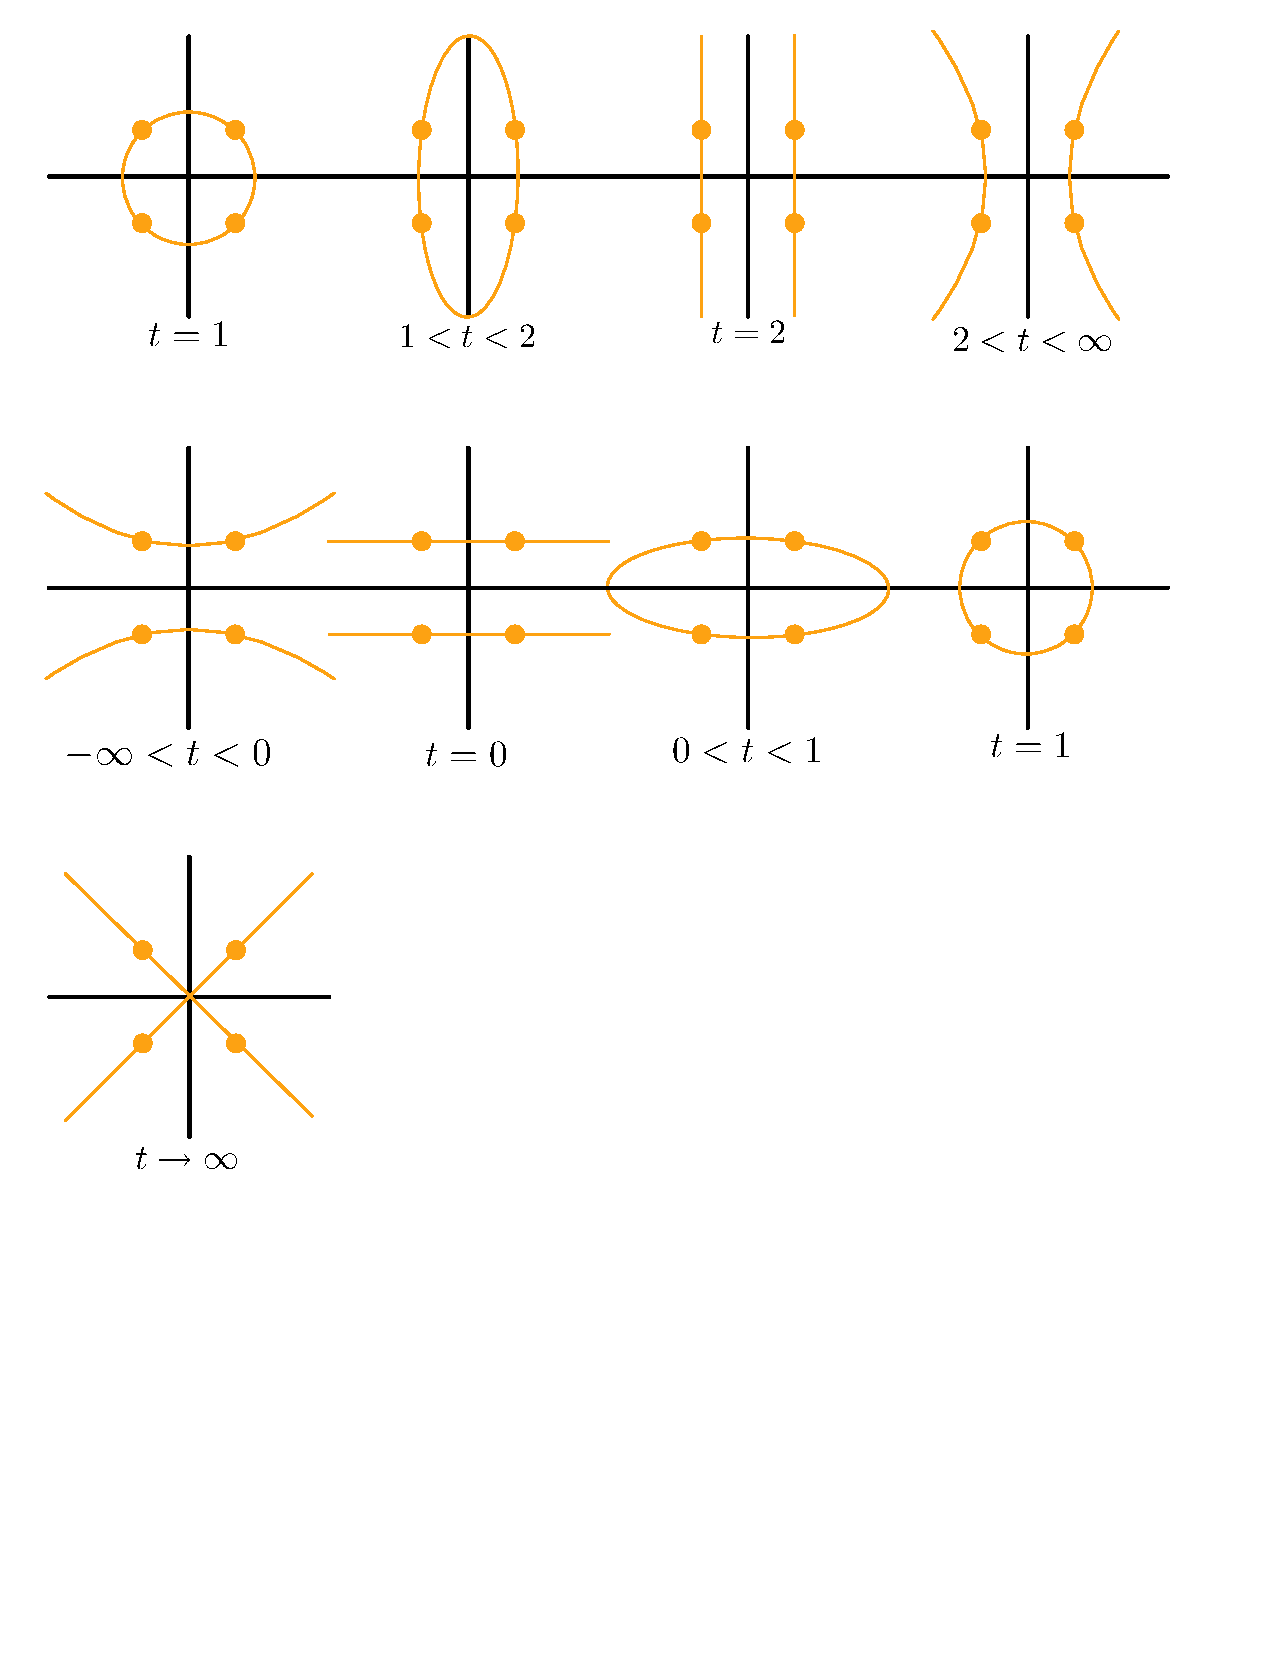
\includegraphics[width=0.3\textwidth, trim= 0.8cm 22.9cm 16cm 0.6cm,clip]{fig1.pdf}
        \label{fig1}
        \caption{One of the quadratic curves passing through our points: $x^2+y^2=2$.}
    \end{figure}
    Ideally we would like to stretch and shrink the circle in order to make it an ellipse. We know ellipses have equations of the form $x^2/a^2+y^2/b^2=1$, but to begin from our circle equation we will instead add coefficients to the equation 
    $$Ax^2+By^2=2.$$
    These coefficients are determined by the points on the curve, we may derive the relation by plugging in a point into the equation:
    $$A(1)^2+B(1)^2=2\To B=2-A\To tx^2+(2-t)y^2=2$$
    where we take $t=A$ to get the last equation.
    We annotate the curves we obtain given different values of $t$:
    \vspace{-0.5em}
    \begin{itemize}
        \begin{multicols}{2}
            \itemsep=-0.4em
        \item $(t=1)$: A circle.
        \item $(1<t<2)$: An ellipse.
        \item $(t=2)$: The pair of lines $x^2=1$.
        \item $(t>2)$: A hyperbola.
        \end{multicols}
    \end{itemize}
    However we are left with one curve which passes through the points in question. To find it we will assume $t$ is non-zero. From our parametric equation we obtain 
    $$tx^2+(2-t)y^2=2\To x^2+o(t)+y^2=\frac{2}{t}\xrightarrow[t\to\infty]{}x^2=y^2$$
    which is the pair of lines $y=\pm x$. Observe that this behavior is independent of the sign of the infinity we are going to. 
    \begin{figure}[h!]
        \centering
        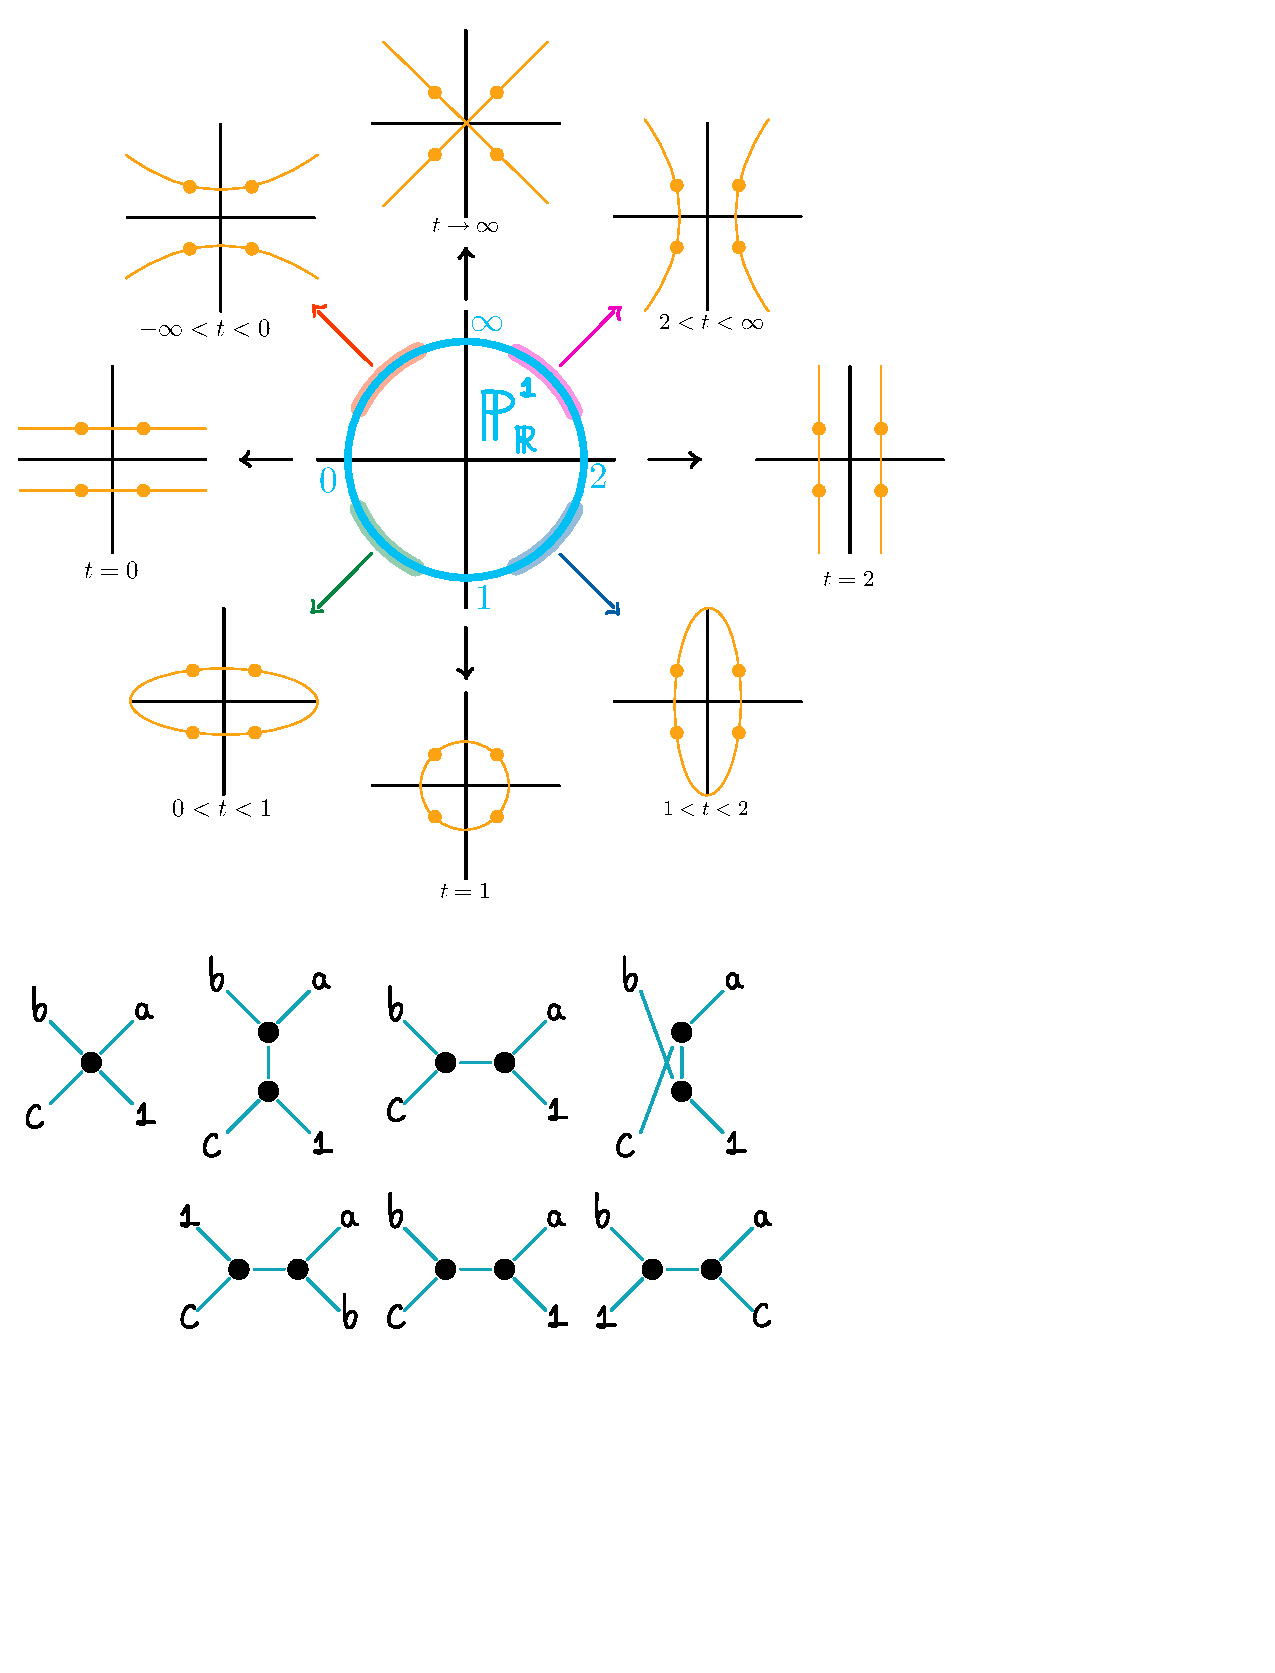
\includegraphics[width=0.8\textwidth, trim= 0.25cm 13.1cm 5.25cm 0.5cm,clip]{fig2.pdf}
        \label{fig2}
        \caption{The projective real line as the moduli space $\ov\cM_{0,4}$.}
    \end{figure}
    In essence what we have seen is that all the quadratic curves passing through our set of points can be parametrized by $\bR\cup\set{\infty}$. Formally:
    \begin{Prop}\label{prop:cM04barIsomP1}
    The moduli space $\ov{\cM}_{0,4}$ can be identified with $\bP^1_\bR$.
    \end{Prop}
    Intuitively the moduli space is a set of parameters. When the points vary \emph{continuously}, the objects they parametrize deform \emph{continuously} as well. What we have done here is not a proof of the previous proposition but it may serve as evidence that it is true.\par 
    To study this space and other spaces which may arise in this fashion, we may ask a question like \emph{how many such curves can we find?} In order to do this, we will address this problem by connecting it with graphs. 
    
    \section{Connection with trees}
    
    As a first approach we could consider an incidence graph where our vertices are the marked points and they are connected if they are in the same component of our curve. However that might produce undesirable results as it could lead to disconnected graphs.
    
    \begin{Def}
    For a point in $\ov{\cM}_{0,X}$ (which represents a curve), we define the \underline{dual tree} to that curve as:
    \begin{itemize}
        \item $V=X\cup I$ where $I$ is the set of irreducible components in our curve. The set $X$ attaches \textbf{labels} to our vertices while the curves are unlabeled.
        \item Vertices in $X$ are not connected between themselves, but $u\in X$ is adjacent to $v\in I$ if $u$ lies in the irreducible component associated to $v$.\par 
        For $u,v\in I$, $uv$ is an edge if the components meet at a nodal singularity.
    \end{itemize}
    \end{Def}
    
    Even though we have defined the dual tree to be a tree, it may not be totally clear why this is the case: %\textbf{buajaja figure \ref{fig2} \ref{fig1}}
    \begin{significant}
        Why should this process generate a tree? Why not a disconnected graph or a cycle?
    \end{significant}
    This follows from the definition because we are talking about \emph{genus $0$} curves. When we admit holes, what we are allowing in the graph is cycles.
    
    \begin{Ex}
    Let us consider the case of $\ov\cM_{0,4}$, our labeled vertices will be 
    $$a=(1,1),\quad b=(-1,1),\quad c=(-1,-1),\quad 1=(-1,-1).$$
    We have different types of trees:
    \begin{enumerate}
        \itemsep=-0.4em
        \item For ellipses and circles, the vertices are ${a,b,c,1}$ or ${\cdot}$, and the edges are of the form $x\cdot$ for $x\in X$. This gives us a $K_{1,4}$ graph.
        \item Hyperbolas have a unique component. In the projective plane, the components are connected at the point corresponding to the \emph{slope of the asymptotes} at infinity, so the dual trees of the hyperbolas are also $K_{1,4}$ graphs.
        \item For $t=0$, there are two unlabeled vertices. $a$ and $b$ are connected to one vertex, while $c$ and $1$ are connected to the other. At infinity, there is a nodal singularity at the point corresponding to the slope of the lines, which means they connect.\par 
        A similar analysis can be done for $t=2$ and $t\to\infty$, and the resulting graph is two copies of $P_3$ connected by their middle vertices.
    \end{enumerate}
    The corresponding trees are shown in the following figure: 
    \begin{figure}[h!]
        \centering
        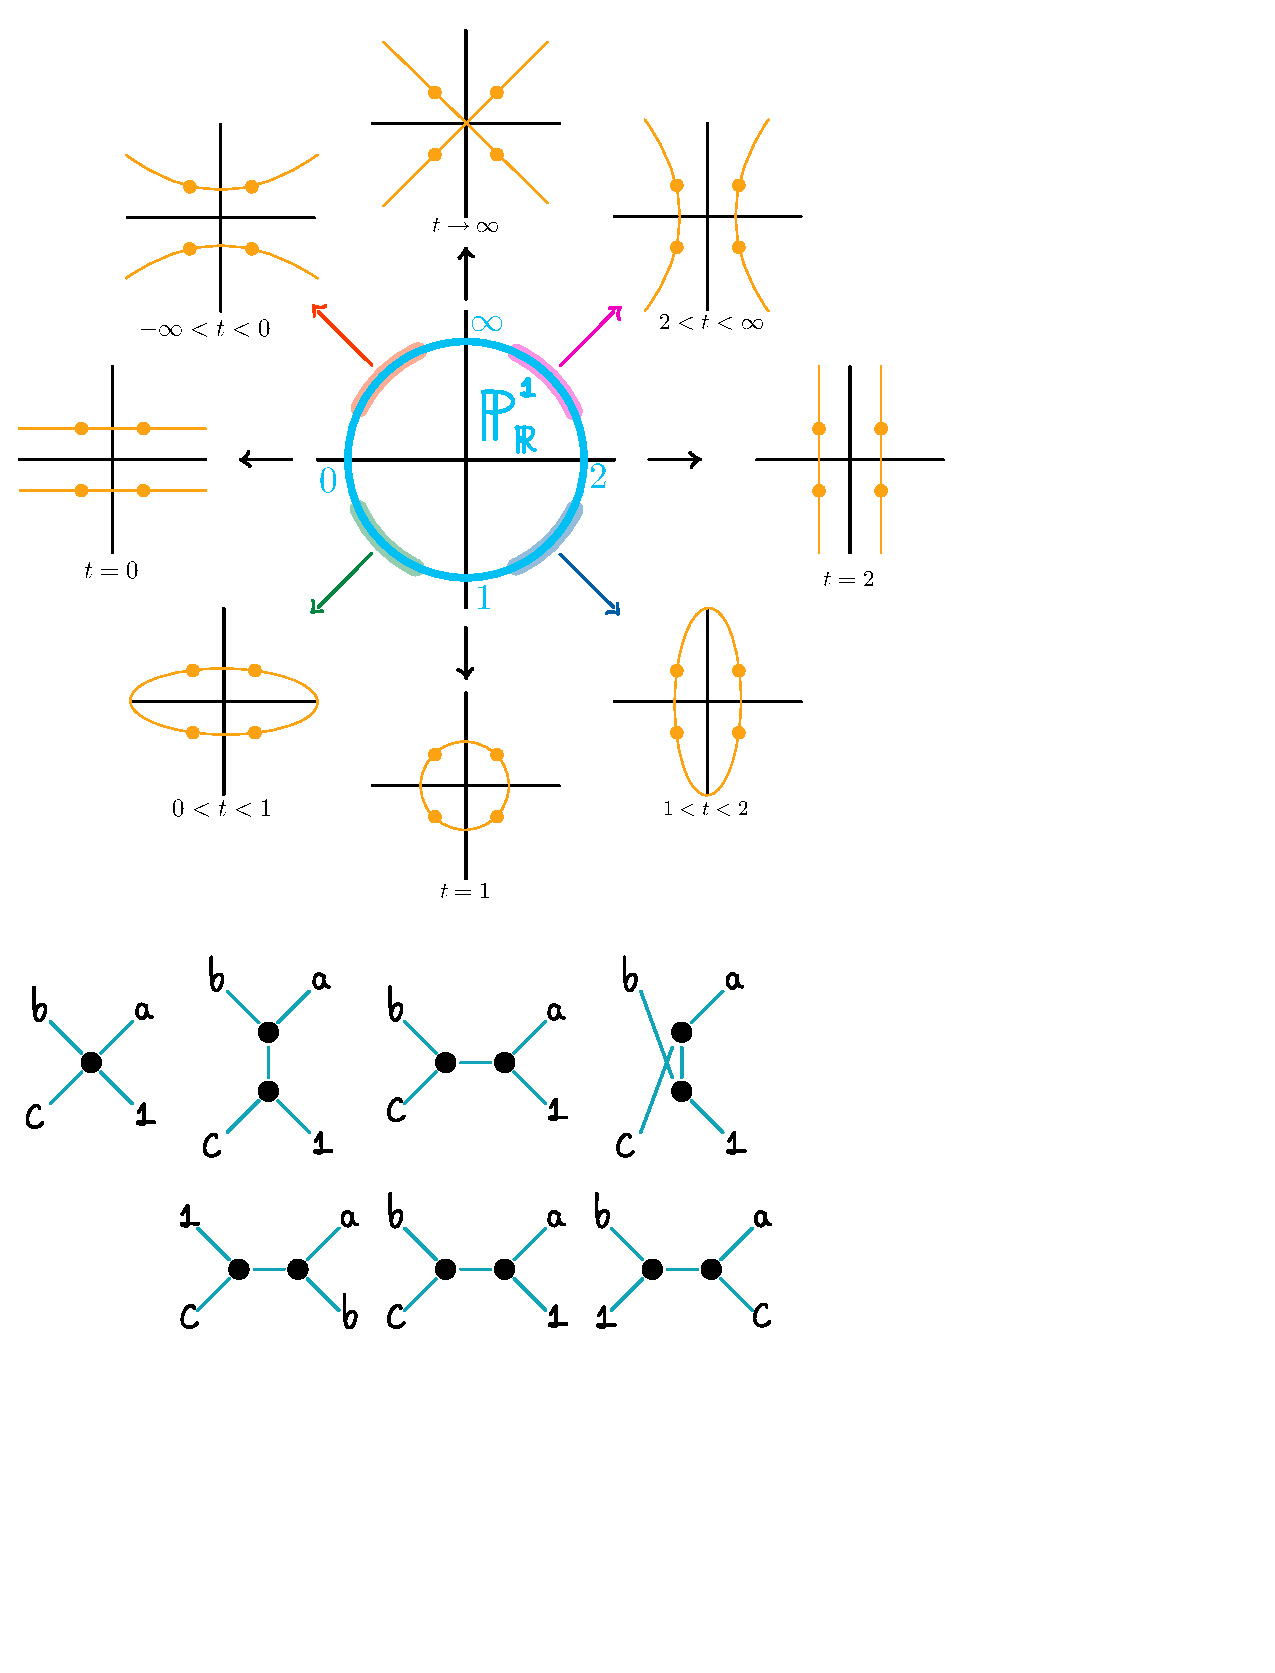
\includegraphics[width=0.8\textwidth, trim= 0.4cm 8.3cm 9cm 16cm,clip]{fig2.pdf}
        \label{fig3}
        \caption{Trees associated to: $(1)$ circles, ellipses and hyperbolas; $(2)$ the curve $y^2=1$; $(3)$ the curve $x^2=1$; and $(4)$ the curve $x^2=y^2$.}
    \end{figure}
    \end{Ex}
    
    \begin{Rmk}
    Look at the degrees of our vertices, there are no vertices of degree 2. If we remove the labels, all the trees besides $(1)$ are isomorphic.\par
    Also notice that when talking about the ellipses and the circle, we did not assign a particular value of $t$ to each of the curves. We just said \emph{an ellipse} or also \emph{an hyperbola}, which means that the whole family of those curves is associated to the particular tree we obtained.
    \end{Rmk}
    
    \begin{Def}
    For a tree $T$ we have that:
    \begin{enumerate}
        \itemsep=-0.4em
        \item $T$ is \underline{trivalent} if all vertices of $T$ have degree $1$ or $3$ and at least one vertex has degree $3$.
        \item $T$ is \underline{at least trivalent} if no vertex of $T$ has degree $2$ and at least one vertex has degree at least $3$.
    \end{enumerate}
    \end{Def}
    
    \begin{Rmk}
    In our graphs, observe that the trees associated to \emph{families} of curves like ellipses and hyperbolas, correspond to \emph{at least trivalent} trees.\par 
    While for the particular cases $t=0$, $t=2$ and $t\to\infty$ we get exactly \emph{trivalent} trees. \emph{This is no coincidence!} The fact that at least trivalent trees correspond to a large number of curves and that the trivalent ones only to a select few.
    \end{Rmk}
    
    \begin{Def}
        The \underline{boundary stratum} corresponding to a tree $T$ is the set of curves whose dual tree is $T$. 
    \end{Def}
    
    \begin{Ex}
    In our example, the boundary stratum of $K_{1,4}$ is $$\obonj{-\infty,0}\cup\obonj{0,2}\cup\obonj{2,\infty}$$
    where we identify $\infty$ with $-\infty$.\par 
    The remaining points $\set{0},\set{2}$ and $\set{\infty}$ are \emph{zero-dimensional} and these are the boundary points which correspond to the trivalent trees.
    \end{Ex} 
    
    The observation that the boundary points correspond to the trivalent trees is key, because knowing this allows us to simplify the problem of counting the boundary points to counting \emph{certain} trivalent trees. In general this result is true:
    
    \begin{Prop}
        The boundary points of $\ov\cM_{0,X}$ correspond to trivalent trees whose leaf set is labeled with $X$. If $X=\set{a,b,c,1,2,\dots,n}$, then the number of boundary points of $\ov\cM_{0,X}$ is $(2n+1)!!$. 
    \end{Prop}
    
    To count the number of leaf-labeled trivalent trees $L_n$ on $n+3$ leaves, we begin with the following small values:
    \begin{itemize}
        \item When $n=0$, there is only one tree, $K_{1,3}$, with a unique labeling of the leaves. So $L_0=1$, which coincides with $(2(0)+1)!!=1$.
        \item When $n=1$, we have two copies of $P_3$ joined by their middle vertices. There are $4!$ ways to label the four leaves without constraints. Accounting for symmetries, we have $L_1=4!/2^3=3$, as pictured in the figure above.
        \item For the next case we are supposed to find $15$ trees. Counting by hand or considering symmetries is not the way to go. We've got to be more creative than that. A question arises:
        \begin{significant}
            Is there a way to obtain the next trees from the old trees?
        \end{significant}
        In essence, we wish to add a new leaf to our graph. Intuitive ways in which we could proceed are:
        \begin{itemize}
            \item Adding the leaf to a leaf vertex. But this actually doesn't work. We add one leaf but we lose one and even worse, now one vertex \textbf{has degree 2}. This means our tree is \textbf{no longer trivalent}.
            \item Adding the leaf to a non-leaf vertex. Indeed we now have a new leaf, but the vertex we added to now has \textbf{degree 4}. So our tree is \textbf{no longer trivalent}.
        \end{itemize}
        Apparently our original ideas won't work. So with a boost of creativity we will instead pop the leaf \emph{out of an edge}:\par
        \begin{figure}[h!]
            \centering
            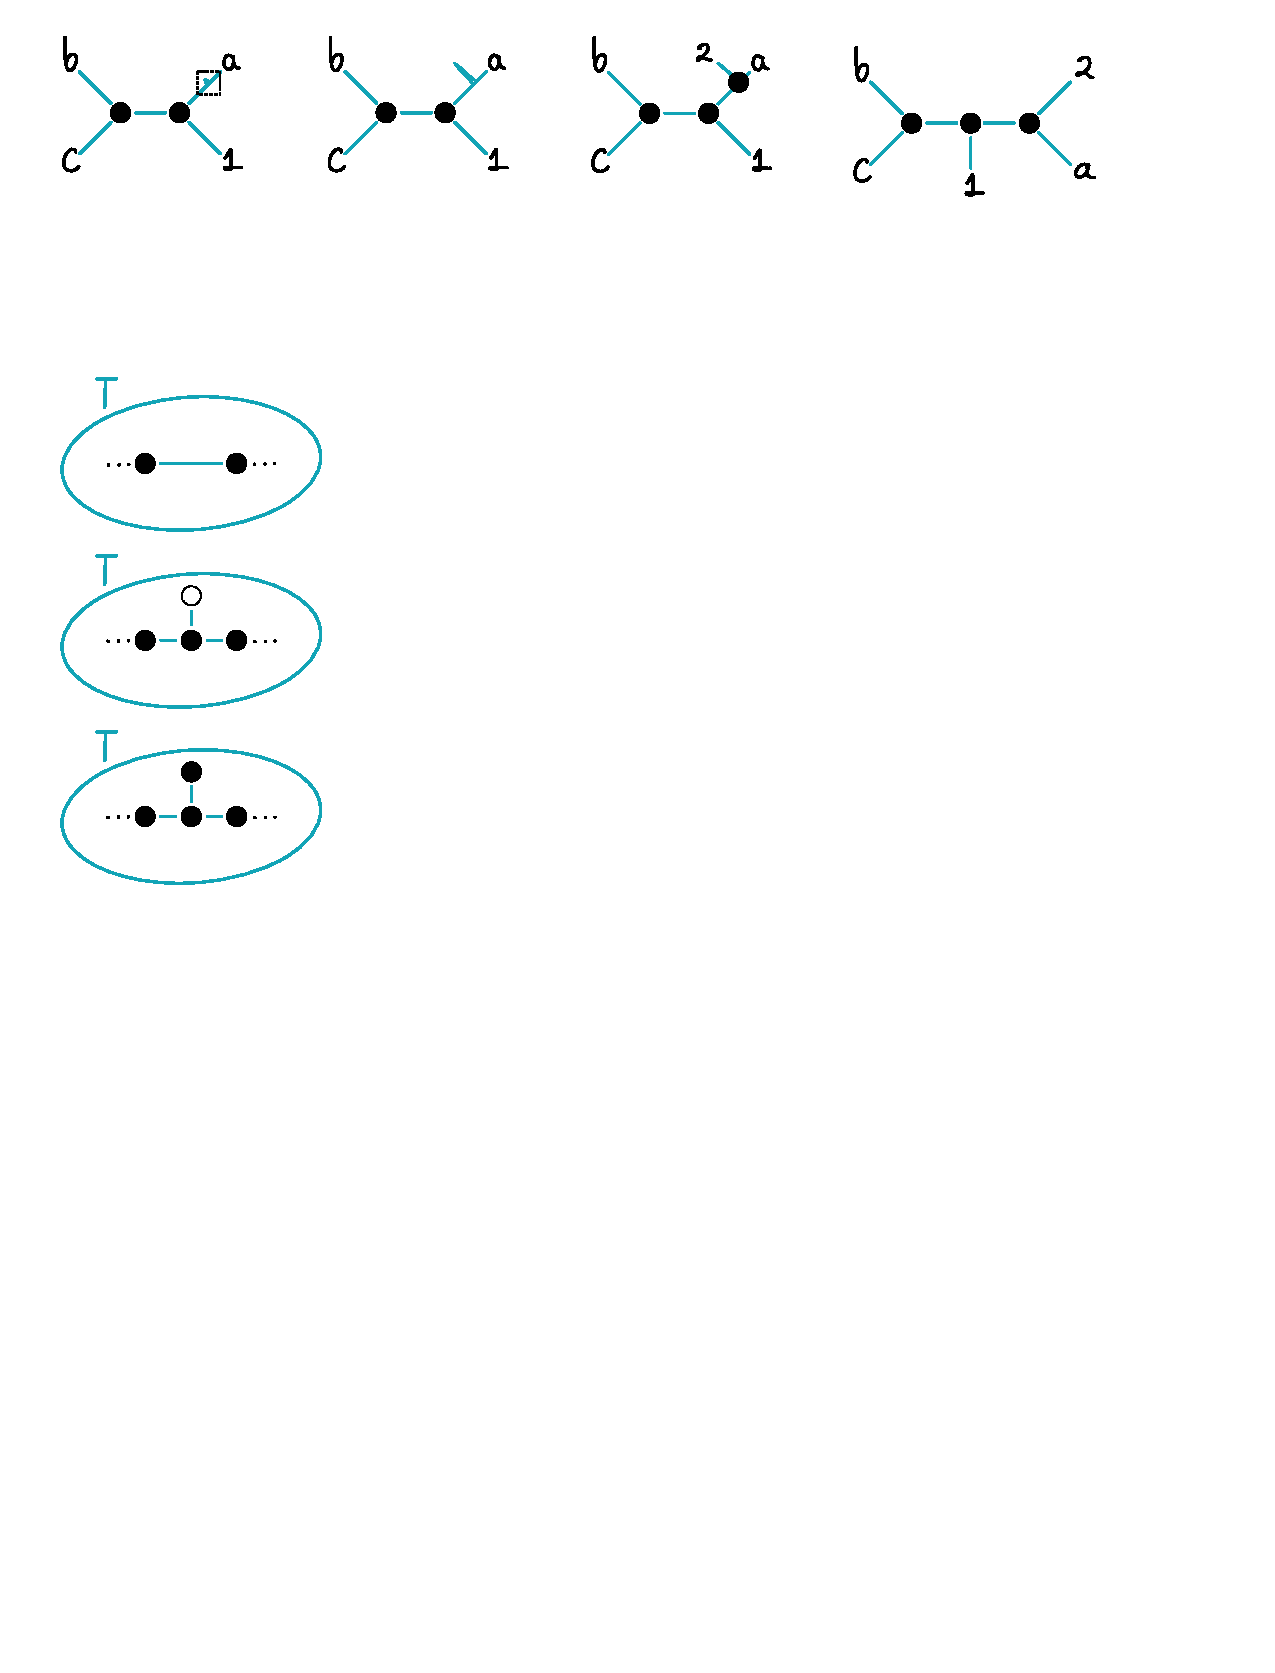
\includegraphics[width=0.8\textwidth, trim= 1cm 25cm 3.05cm 0.65cm,clip]{fig3.pdf}%LDRU
            \label{fig4}
            \caption{\emph{Popping} a leaf out of an edge to form a new trivalent tree.}
        \end{figure}
        Note that adding a leaf to an edge creates a new vertex with degree $3$ and adds a new leaf to the tree. There is no constraint on the number of vertices in a trivalent tree, so we can add as many new leaves as we want.\par 
        Back to our three trees, each one has 5 edges which means there are 5 possible ways to add a labeled leaf. This gives us a total of 15 ways to form a 5-leaved labeled trivalent tree from the previous ones. Thus, $L_2=15$, which is equal to $(2\Cdot2+1)!!=1\Cdot3\Cdot5$.
        \item For $n=3$, we count leaf-labeled trivalent trees with $6$ leaves. Each of our $15$ previous trees has $7$ edges to which we can adjoin a new labeled leaf. For each of the trees, these are different possibilities. So in total we have $7\Cdot L_2=105$ new trees. 
    \end{itemize}
    
    We formalize this strategy using a couple of lemmas:
    
    \begin{Lem}
    The number of edges $E_n$ on a trivalent tree with $n+3$ leaves satisfies the recursion:
    $$E_n=E_{n-1}+2,\quad E_0=3$$
    which means that $E_n=2n+3$.
    \end{Lem}
    
    \begin{ptcbp}
        We will proceed using induction. The base cases have been discussed earlier, so now we will use an $(n-1)+3=n+2$ leaved trivalent tree as a starting point.\par 
    To add a new leaf while preserving the trivalent property, we add a new vertex to an existing edge and attach the leaf to that vertex. This process creates two new edges: 
    \begin{itemize}
        \item One edge which was split in two by the addition of the new vertex in the middle.
        \item Another one created by attaching the leaf to the new vertex.
    \end{itemize}
      This means that the number of edges increased by two and the degree of the new vertex is $3$, so $E_n=E_{n-1}+2$ as desired. The recursion can be solved using the initial condition to obtain $E_n=(2n+3)$ for all $n$.
    \end{ptcbp}
    
    \begin{Lem}
    The number of leaf-labeled trivalent trees with $n+3$ leaves, $L_n$, satisfies the recursion 
    $$L_{n}=E_{n-1}L_{n-1},\quad L_0=1.$$ 
    \end{Lem}
    
    \begin{ptcbp}
        The base cases have been proven in the previous discussion. So for an $(n+2)$-leaved tree, we have ${a,b,c,1,2,\dots,n-1}$ as the labels of our leaves.\par 
        Adding the leaf labeled $n$ can be done in $E_{n-1}$ ways because we may attach it to any of the existing edges. Each of these new trees has a unique set of labels, and there are $L_{n-1}$ such trees. Therefore, there are $E_{n-1}L_{n-1}$ new leaf-labeled trivalent trees.\par 
        Solving the recursion we have $L_n=(2n+1)L_{n-1}$ which means that 
        $$L_n=(2n+1)(2n-1)(2n-3)\dots=(2n+1)!!.$$
    \end{ptcbp}
    
    With these results in hand the proposition is immediately true. The fact the boundary points correspond to the trivalent trees is a consequence of the fact that automorphisms of $\bP^1$ are determined by $3$ points.
    
    \section{Understanding the moduli space}
    
    In the previous sections, we have explored the concept of trivalent trees and their relationship to curves and the moduli space $\ov{\cM}_{0,4}$. But what exactly is this space? Our aim now is to provide a concrete explanation of $\ov{\cM}_{0,n}$, and discuss its significance in our understanding of trivalent trees and beyond.
    
    \begin{Def}
        The \underline{moduli space} $\cM_{0,n}$ parametrizes ordered $n$-tuples of distinct points in $\bP^1$ up to \emph{projective equivalence}. Two arrays of points $(p_1,\dots,p_n),\ (q_1,\dots,q_n)$ are equivalent when 
        $$\exists T\in\PGL_2\left[(q_1,\dots,q_n)=(Tp_1,\dots,Tp_n)\right].$$
    \end{Def}
    
    In our case $\cM_{0,4}$ can be seen to be the set of \emph{equivalence classes} of arrays $(p_1,\dots,p_4)$ with $p_i\in\bP^1$. 
    
    \begin{Rmk}
        Drawing an analogy with matrices, where the row-reduced echelon form serves as a canonical representative of the equivalence class of row-equivalent matrices, we seek a similar notion of canonical representation for the moduli space $\cM_{0,4}$.
    \end{Rmk}
    
    \begin{Prop}
        Any projective transformation $T\in\PGL_2$ is determined by where it maps $0,1$ and $\infty$. 
    \end{Prop}
    
    The proof of this fact is a basic computation in linear algebra.
    
    \begin{Rmk}
        Before we proceed with the proof, it is important to note that the projective transformation we will derive maps $0$, $1$, and $\infty$ to three distinct points $p_1$, $p_2$, and $p_3$, respectively. This transformation's inverse will serve as the canonical representative of the equivalence class, as it maps $p_1$, $p_2$, and $p_3$ back to $0$, $1$, and $\infty$, respectively.
    \end{Rmk}
    
    \begin{ptcbp}
        Assigning coordinates we have 
        $$0=[0:1],\quad 1=[1:1],\quad \infty=[1:0].$$
        Now suppose $T=\twobytwo{t_{11}}{t_{12}}{t_{21}}{t_{22}}$ is a projective transformation and $p,q,r$ are points in $\bP^1$ such that
        $$
        \left\lbrace
        \begin{aligned}
            &T[1:0]=p=[p_1:p_2]\\
            &T[0:1]=q=[q_1:q_2]\\
            &T[1:1]=r=[r_1:r_2]
        \end{aligned}
        \right.
        $$
        From the first two equations we have that 
        $$\twobyone{t_{11}}{t_{21}}=m_1\twobyone{p_1}{p_2},\quad\text{and}\quad\twobyone{t_{12}}{t_{22}}=m_2\twobyone{q_1}{q_2}\quad\text{for some}\quad m_1,m_2\neq 0$$
        which means that the columns of $T$ are proportional to $p$ and $q$ and to determine $T$ we are only required to determine $m_1$ and $m_2$. Replacing these entries into the matrix and considering the last equation we have 
        \begin{align*}
            \twobytwo{m_1p_1}{m_2q_1}{m_1p_2}{m_2q_2}\twobyone{1}{1}=m_3\twobyone{r_1}{r_2}&\To \left\lbrace
        \begin{aligned}
            &m_1p_1+m_2q_1=m_3r_1,\\
            &m_1p_2+m_2q_2=m_3r_2,
        \end{aligned}
        \right.\\
        &\To \twobytwo{p_1}{q_1}{p_2}{q_2}\twobyone{m_1}{m_2}=\twobyone{m_3r_1}{m_3r_2}.
        \end{align*}
        The last matrix's columns are linearly independent because they are the image of two l.i. vectors under a linear transformation. This means that we may recover $(m_1,m_2)$ by inverting that matrix:
        $$\twobyone{m_1}{m_2}=m_3\twobytwo{p_1}{q_1}{p_2}{q_2}^{-1}\twobyone{r_1}{r_2}.$$
        This information determines $T$ up to a scalar multiple $m_3$ which means that projectively, we have determined $T$.
    \end{ptcbp}
    
    With the proposition in hand we may map the first $3$ points of our array to the special points $0,1,\infty$, and let the last one map to an arbitrary but fixed $t$:
    $$(Tp_1,\dots,Tp_4)=(0,1,\infty,t),\quad t\in\bP^1.$$
    At the level of equivalence classes this means:
    $$[(\bP^1,(p_1,\dots,p_4))]=[(\bP^1,(0,1,\infty,t))]$$
    and so every equivalence class of points is determined by a unique $t\in\bP^1$.
    
    \begin{figure}[h!]
        \centering
        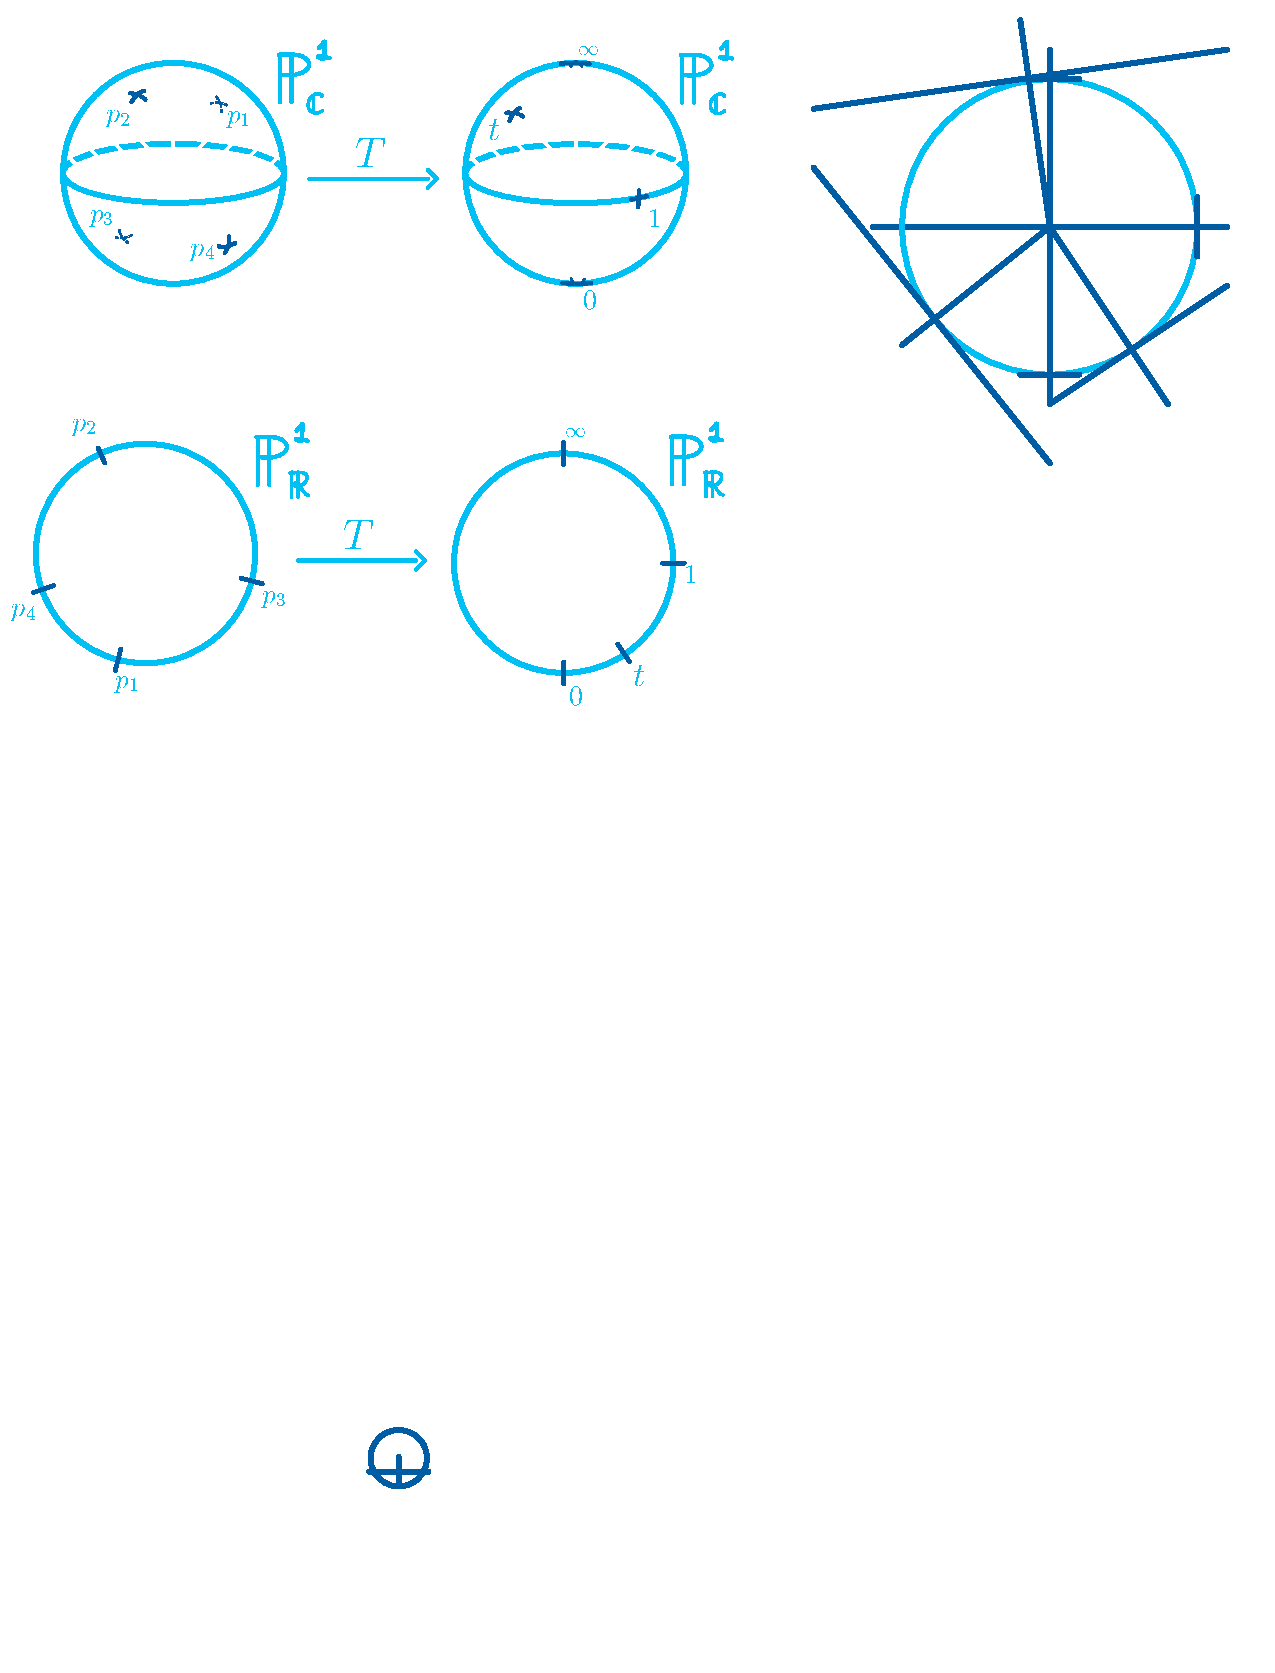
\includegraphics[width=0.8\textwidth, trim= 0.17cm 16.37cm 9.325cm 7.075cm,clip]{fig4.pdf}%LDRU
        \label{fig5}
        \caption{A projective transformation $T$ sending the tuple $(p_1,\dots,p_4)$ to its corresponding representative in the moduli space $\cM_{0,4}$.}
    \end{figure}
    
    \begin{Rmk}
    Recall that in the definition of the moduli space, we stated that the points $(p_1,\dots,p_4)$ should be \textbf{distinct}! So this means that $t$ is not in the whole of $\bP^1$, $t$ can't be $0,1$ nor $\infty$. 
    \end{Rmk}
    
    The previous discussion proves the following result.
    
    \begin{Prop}
        The moduli space $\cM_{0,4}$ is isomorphic to $\bP^1\less\set{0,1,\infty}$.
    \end{Prop}
    
    The following is the concrete definition of the closure of $\cM_{0,n}$. We can intuitively see that the missing points in the closure are $0$, $1$ and $\infty$.
    
    \begin{Def}
        The space $\ov{\cM}_{0,n}$ parametrizes \emph{stable $n$-pointed rational curves}. And one of those curves is a tuple $(\cC,p_1,\dots,p_n)$ such that:
        \begin{enumerate}
            \itemsep=-0.4em
            \item $\cC$ is a connected curve of arithmetic genus 0 with at worst simple nodal singularities.
            \item The points $p_1,\dots,p_n$ are distinct and non-singular on $\cC$.
            \item Each irreducible component of $\cC$ has at least $3$ special points (be it marked points or nodes).
        \end{enumerate}
    \end{Def}
    
    The fact that nodal singularities may appear, allows us to have $t$ equal one of the missing points. And, although before it seemed that the point $t$ was not varying throughout $\bP^1$, it actually was under the guise of projective equivalence.
    
    \section{Conclusion}
    
    Enumerative geometry poses a wealth of interesting questions, some of which have yet to be answered. Our understanding of moduli spaces has increased while studying the original question in this paper. The task now is to continue studying more general moduli spaces, by increasing the number of marked points or by increasing the genus of the curves. While the combinatorics used to describe non-zero genus curves is currently very complicated, the author hopes to explore these topics in the future.
    
    \section{Acknowledgements}
    
    First and foremost, the author would like to thank \textbf{you} for reading. Thanks also to \textbf{Maria Gillespie} for encouraging students to do projects at the end of the semester and for her guidance during the writing process. Thanks to \textbf{Mark Shoemaker} for his help by answering questions about the algebraic background needed to understand the moduli space. And last but not least, thanks to \textbf{the author's family and friends} for their unwavering support, even from over 3000km away. 
    
%%%%%%%%%%%% Contents end %%%%%%%%%%%%%%%%
\ifx\nextra\undefined
\printindex
\else\fi
\nocite{*}
\bibliographystyle{plain}
\bibliography{bibiProyCombi2.bib}
\end{document}